% Autor: Leonhard Segger, Alexander Neuwirth
% Datum: 2017-10-30
\documentclass[
	% Papierformat
	a4paper,
	% Schriftgröße (beliebige Größen mit „fontsize=Xpt“)
	12pt,
	% Schreibt die Papiergröße korrekt ins Ausgabedokument
	pagesize,
	% Sprache für z.B. Babel
	ngerman
]{scrartcl}

% Achtung: Die Reihenfolge der Pakete kann (leider) wichtig sein!
% Insbesondere sollten (so wie hier) babel, fontenc und inputenc (in dieser
% Reihenfolge) als Erstes und hyperref und cleveref (Reihenfolge auch hier
% beachten) als Letztes geladen werden!

\usepackage{tikz}
\usetikzlibrary{calc,patterns,angles,quotes} % loads some tikz extensions\usepackage{tikz}
\usetikzlibrary{babel}

% Silbentrennung etc.; Sprache wird durch Option bei \documentclass festgelegt
\usepackage{babel}
% Verwendung der Zeichentabelle T1 (Sonderzeichen etc.)
\usepackage[T1]{fontenc}
% Legt die Zeichenkodierung der Eingabedatei fest, z.B. UTF-8
\usepackage[utf8]{inputenc}
% Schriftart
\usepackage{lmodern}
% Zusätzliche Sonderzeichen
\usepackage{textcomp}

% Mathepaket (intlimits: Grenzen über/unter Integralzeichen)
\usepackage[intlimits]{amsmath}
% Ermöglicht die Nutzung von \SI{Zahl}{Einheit} u.a.
\usepackage{siunitx}
% Zum flexiblen Einbinden von Grafiken (\includegraphics)
\usepackage{graphicx}
% Abbildungen im Fließtext
\usepackage{wrapfig}
% Abbildungen nebeneinander (subfigure, subtable)
\usepackage{subcaption}
% Funktionen für Anführungszeichen
\usepackage{csquotes}
\MakeOuterQuote{"}
% Zitieren, Bibliografie
\usepackage[sorting=none]{biblatex}


% Zur Darstellung von Webadressen
\usepackage{url}
%chemische Formeln
\usepackage[version=4]{mhchem}
% siunitx: Deutsche Ausgabe, Messfehler getrennt mit ± ausgeben
\usepackage{floatrow}
\floatsetup[table]{capposition=top}
\usepackage{float}
% Verlinkt Textstellen im PDF-Dokument
\usepackage[unicode]{hyperref}
% "Schlaue" Referenzen (nach hyperref laden!)
\usepackage{cleveref}
\sisetup{
	locale=DE,
	separate-uncertainty
}
\bibliography{BA-C-04_V01_13-05-2019_References}

\begin{document}

	\begin{titlepage}
		\centering
		{\scshape\LARGE Versuchsbericht zu \par}
		\vspace{1cm}
		{\scshape\huge V01 - NaI- und Ge-Detektor \par}
		\vspace{2.5cm}
		{\LARGE Gruppe BA-C-04 \par}
		\vspace{0.5cm}

		{\large Alexander Neuwirth (E-Mail: a\_neuw01@wwu.de) \par}
		{\large Leonhard Segger (E-Mail: l\_segg03@uni-muenster.de) \par}
		\vfill

		durchgeführt am 13.05.2019\par
		betreut von\par
		{\large Axel Buß}

		\vfill

		{\large \today\par}
	\end{titlepage}
	\tableofcontents
	\newpage

	\section{Kurzfassung}
	% Hypothese	und deren Ergebnis, wenn Hypothese ist, dass nur Theorie erfüllt, sagen: Erwartung: Theorie aus einführung (mit reflink) erfüllt
	% Ergebnisse, auch Zahlen, mindestens wenn's halbwegs Sinn ergibt
	% Was wurde gemacht
	% manche leute wollen Passiv oder "man", manche nicht
	In diesem Versuch sollen Messungen mit zwei verschiedene Detektoren für Gamma-Strahlung durchgeführt werden.
	Auf Basis dieser Messungen werden dann qualitative Vergleiche der Detektortypen durchgeführt.
	Verwendet wird einerseits ein thallium-aktivierter Natrium-Iodid-Kristall (NaI(TI)) als Szintallationsdetektor und andererseits ein lithium-kompensierter Germanium-Halbleiterdetektor (Ge(Li)).


  \section{Theorie}
	% wdh. Texte
	% wdh. Besprechung

	% Gamma-Entstehung: Was ist das, wie entsteht das
	% Welche Zerfälle gibt es
	% Was braucht man für Gammazerfall? Halt Zerfall in angeregtes Niveau
	\subsection{$\gamma$-Strahlung}
	$\gamma$-Strahlung ist elektrische Strahlung, die sich entweder über den Energiebereich oder durch die Entstehungsart definieren lässt.
	Energetisch liegt die $\gamma$-Strahlung in der Regel über der Röntgenstrahlung, also etwa ab \SI{100}{keV}.
	Sie entsteht dadurch, dass nach radioaktiven Zerfällen anderer Art der Kern in einem angeregten Zustand vorliegt, der dann durch Aussenden von elektromagnetischer Strahlung ($\gamma$-Strahlung) in den Grundzustand übergeht.
	Die Zerfallsschemata einiger der in diesem Versuch verwendeten Proben sind in \cref{fig_zerfallsschemata} dargestellt.
	Es findet wie beschreieben jeweils ein $\beta$-Zerfall (bzw. Elektroneneinfang) in ein angeregtes Niveau statt.
	Das angeregte Niveau geht dann entweder direkt oder über Zwischenniveaus in den Grundzustand über und $\gamma$-Strahlung wird frei.

	Neben dem $\gamma$-Zerfall gibt es $\alpha$-, $\beta$-Zerfall und Elektroneneinfang, bei denen respektive ein Heliumkern, Elektron oder Positron ausgesandt werden und sich Ladung- bzw. Nukleonenzahl ändern.

	Die folgende Reaktionsgleichung entspricht dem $\alpha$-Zerfall:

	\begin{equation}
		\label{eq_alphazerfall}
		 _{Z}^{A}\text{X} \rightarrow _{Z-2}^{A-4}\text{Y} + _{2}^{4}\text{He} \Delta E
	\end{equation}

	Beim $\beta$-Zerfall trennt man in:

	\begin{align}
		\label{eq_beta-minus}
		\beta^-: \quad & _{Z}^{A}\text{X} \rightarrow _{Z+1}^{A}\text{Y} + \text{e}^- + \bar{\nu_{\text{e}}}\\
		\beta^+: \quad & _{Z}^{A}\text{X} \rightarrow _{Z-1}^{A}\text{X} + \text{e}^+ + \nu_{\text{e}}
	\end{align}

	Beim Elektroneneinfang findet aufgrund der Überlagerung der Wellenfunktionen von Hüllenelektronen und Kern im Kern die folgende Umwandlung statt:
	\begin{equation}
		\label{eq_elec_cap}
		\text{e}^- + \text{p} \rightarrow \text{n} + \nu_{\text{e}}
	\end{equation}

	\begin{figure}[H]
			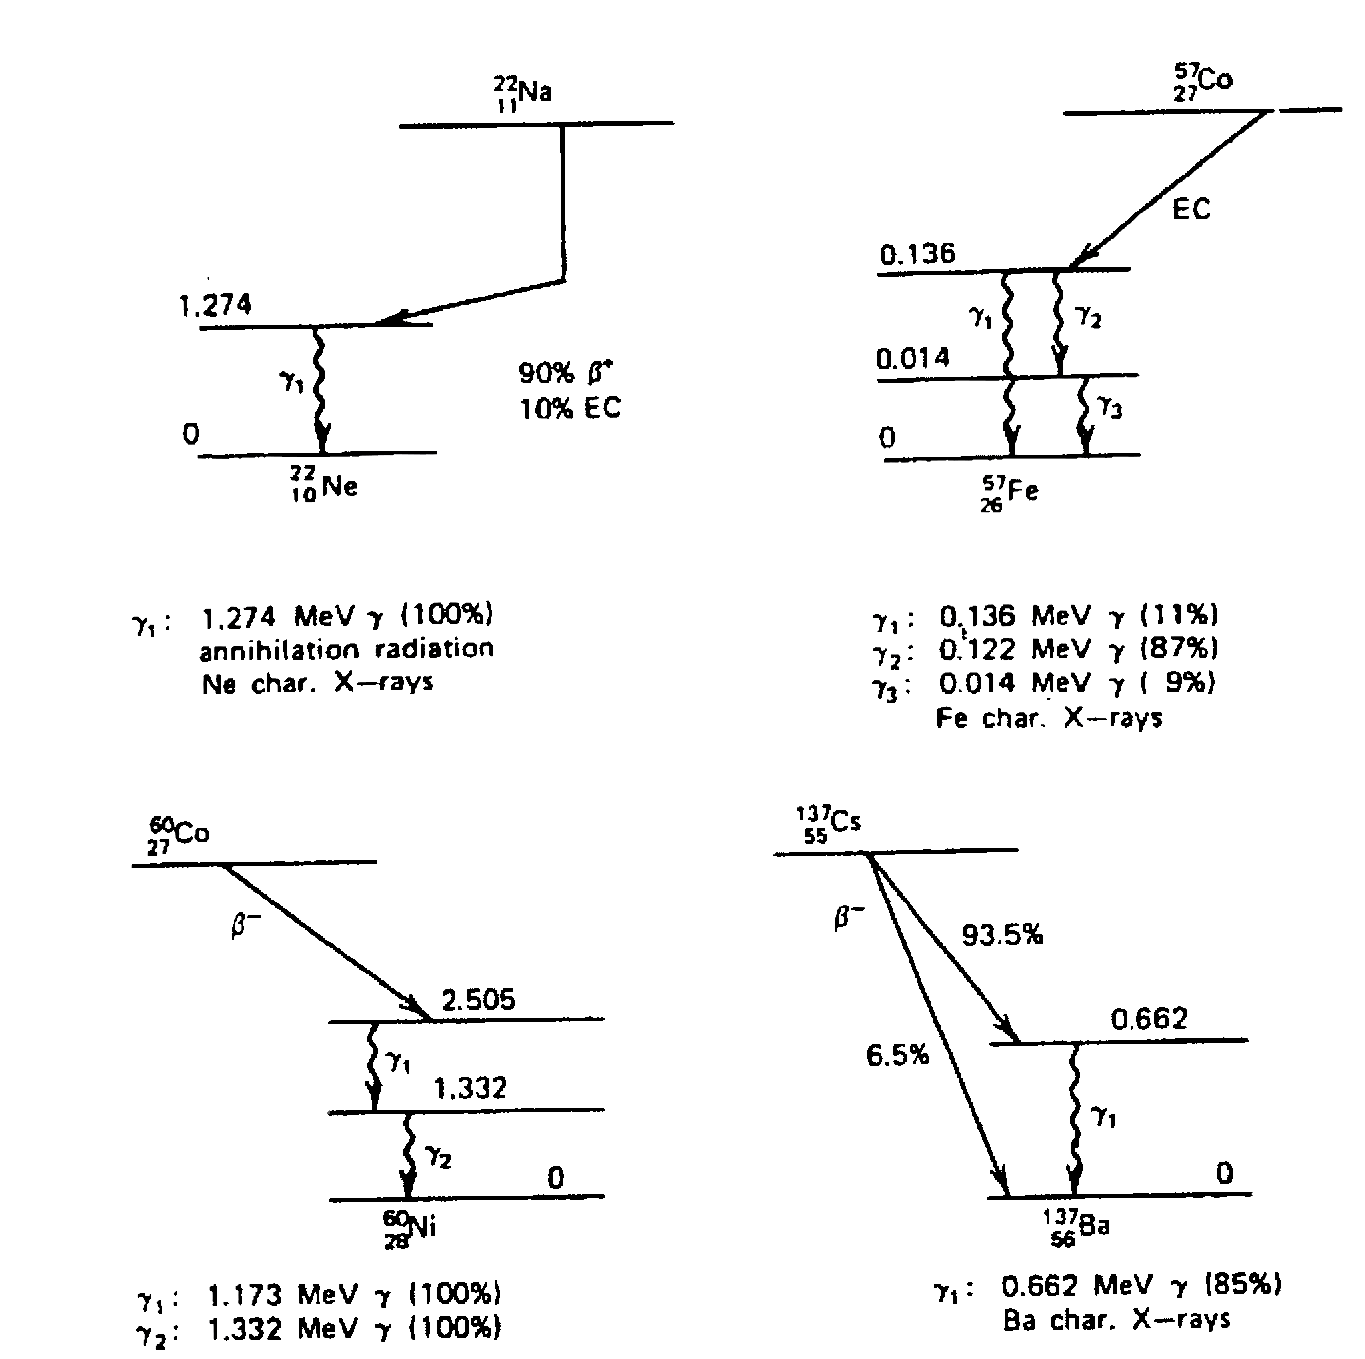
\includegraphics[width= 1 \linewidth]{charts/Zerfallsschemata}
			\caption{
				Zerfallsschemata der relevanten Zerfälle. %TODO
				\cite{Anleitung}
			}
			\label{fig_zerfallsschemata}
	\end{figure}

	\subsection{Wechselwirkung mit Materie}
	% was ist die Schwierigkeit
	%TODO Comptonedge-Gedöns siehe der link?

	Die Detektion von $\gamma$-Strahlung ist dadurch gegenüber der Detektion von Strahlung aus anderen Zerfällen erschwert, als dass sie keine Ladung besitzt.
	Wenn man zusätzlich zum reinen Nachweis der Strahlung noch Information über Zeitpunkt des Auftreffens auf den Detektor, Intensität und Energie erhalten möchte, muss man sich mit der Wechselwirkung der Strahlung mit Materie auseinandersetzen und auf Basis dessen einen Detektor konstruieren.

	Da $\gamma$-Strahlung im Allgemeinen geringe Wechselwirkung mit Materie zeigt, muss für eine zielführende Messrate ein Stoff mit hoher Dichte (ein Festkörper) verwendet werden.

	\begin{figure}[H]
			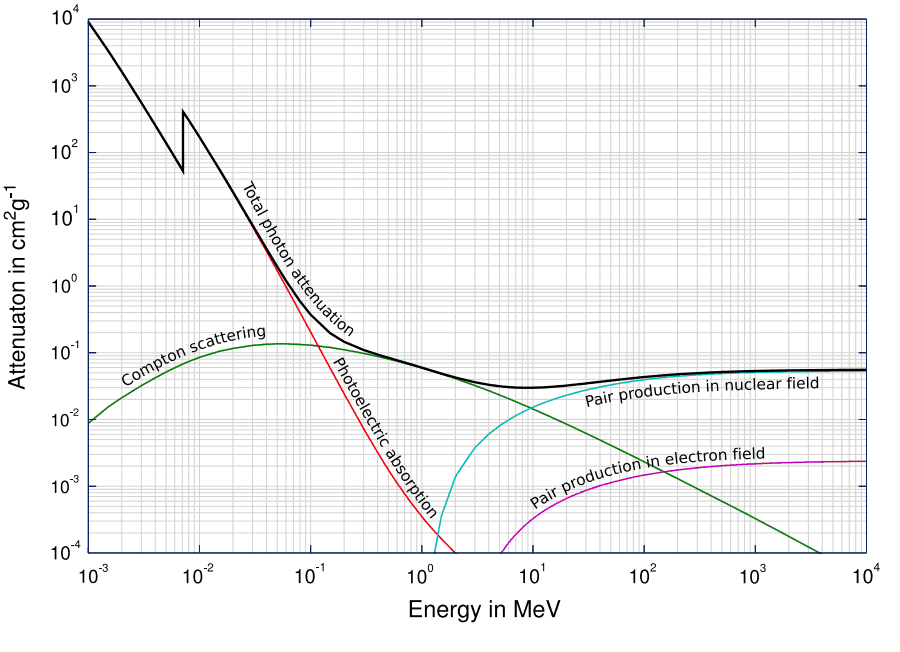
\includegraphics[width= 1 \linewidth]{charts/interaktion}
			\caption{
				Wirkungsquerschnitt von Photonen in Materie in Abhängigkeit von der Energie aufgeteilt in Compton-Effekt, photoelektrischen Effekt und Paarbildung sowie der Gesamtwirkungsquerschnitt.
				\cite{atomkraft}
			}
			\label{fig_wirkunsquerschnitt_gamma}
	\end{figure}

	In \cref{fig_wirkunsquerschnitt_gamma} ist der Wirkungsquerschnitt von Photonen in Materie durch die verschiedenen Effekte dargestellt.
	Außerdem steigt die Wechselwirkungwahrscheinlichkeit mit der Ladungszahl der Materie, durch die sich das Photon bewegt.

	% Abhängigkeit von Wirkungsquerschnitt von Energie? andere Faktoren?

	\subsubsection{Photoeffekt}
	% Vernachlässigung der Bindungsenergie `bei Photoeffekt möglich?
	% Abhängigkeit von Wirkungsquerschnitt von Energie für Photoeffekt?
	% warum sind da Stufen im Wirkungsquerschnitt?
	Beim Photoeffekt trifft ein $\gamma$-Photon seine Energie an ein Hüllenelektron im Detektor ab und wird dabei absorbiert.
	Das Hüllenelektron wird aus der Atomhülle gelöst, wofür Energie des Photons aufgewendet wird, und bewegt sich dann mit der Restenergie als kinetischer Energie durch die Materie.
	Die Energie der $\gamma$-Strahlung ($\ge \SI{100}{keV}$) ist dabei so deutlich größer als die Ionisierungsenergie (Größenordnung von wenigen \si{}{eV}), dass angenommen werden kann, dass alle Energie der $\gamma$-Strahlung in kinetische Energie umgesetzt wird.
	Für den Wirkungsquerschnitt gilt nach \cite{queensu}:

	\begin{equation}
		\label{eq_photo_wirk}
		\sigma \propto Z^5 E_\gamma^{-\frac{7}{2}}
	\end{equation}

	Außerdem hängt der Wirkungsquerschnitt in der $\gamma$-Energie von den Ionisationskanten ab, sodass eine Stufenform entsteht, da der Wirkungsquerschnitt ansteigt, wann immer die Ionisationsenergie einer weiteren Schale erreicht wird.

	\subsubsection{Comptoneffekt}

	Beim Comptoneffekt streut ein $\gamma$-Photon mit einem freien (oder quasi-freien) Elektron.
	Dabei ändern sich Energie und Bewegungsrichtung des Photons, da Energie auf das Elektron übertragen wird und eine Ablenkung stattfindet.
	Dies ist in \cref{fig_Compton} dargestellt.
	Der Energieübertrag auf das Elektron beträgt:
	\begin{equation}
		\label{eq_compton_energie}
		E_\text{e} = E_\gamma \left[ 1 - \frac{1}{1+(E_\gamma /M_\text{e} c^2)(1-\cos \varphi)} \right]
	\end{equation}

	Das Spektrum ist kontinuierlich, da in Abhängigkeit von der Geometrie des Stoßes ein beliebiger Anteil der Energie des Photons (bis zu einer Maximalenergie) an das Elektron übertragen werden kann.
	%TODO warum U-förmig?

	\begin{figure}[H]
			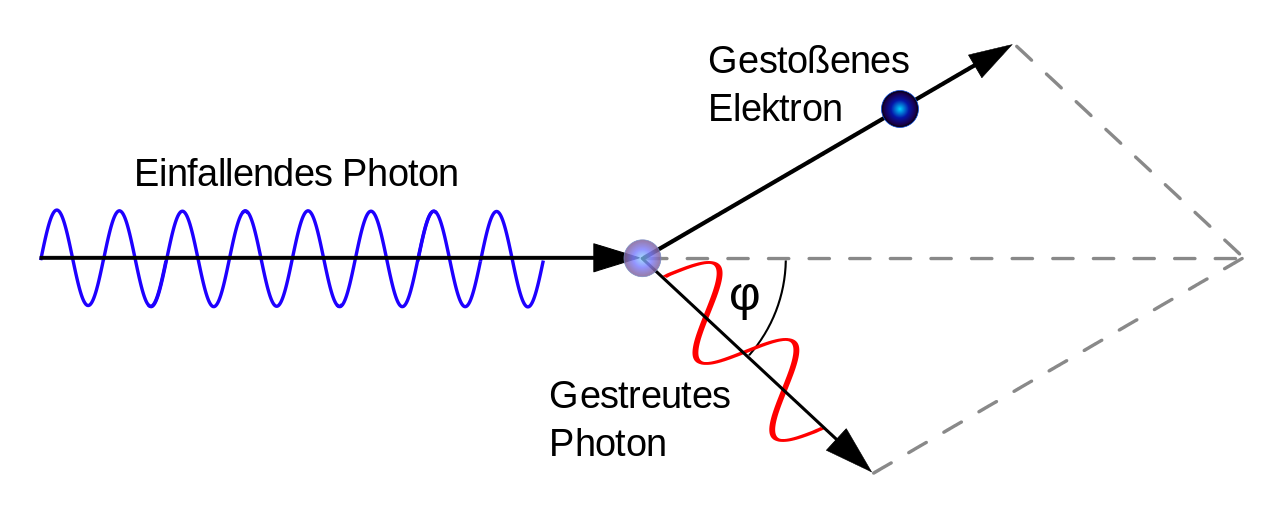
\includegraphics[width= 0.5 \linewidth]{charts/Comptonstreuung}
			\caption{
				Schematische Darstellung des Compton-Effekts.
				\cite{comptonwiki}
			}
			\label{fig_Compton}
	\end{figure}

	\subsubsection{Paarbildung}
	% waas ist für Paarbildung ötig?
	% Sekundäreffekte bei Paarbildung?
	In Wechselwirkung mit einem Atom (oder anderen Teilchen) kann ein $\gamma$-Photon die Entstehung eines Elektron-Positron-Paares hervorrufen.
	Dafür muss es mindestens die Ruheenergie des Teilchenpaares (\SI{1022}{keV}) besitzen.
	Das Photon wird dabei vernichtet und die überschüssige Energie geht in kinetische Energie der Reaktionsprodukte über.

	Das dabei entstandene Positron wird durch Wechselwirkung mit dem Rest der Probe unter Aussendung von Bremsstrahlung abgebremst.
	Wenn es ausreichend stark abgebremst ist, kann es mit einem Elektron in der Probe das instabile Positronium bilden.
	Beim Positronium unterscheidet man je nach Spinausrichtung von Positron und Elektron in Parapositronium ($S=0$) und Orthopositronium ($S=1$).
	Aufgrund von Spin- und Impulserhaltung zerfällt Orthopositronium in eine ungerade Anzahl Photonen, die mindestens \num{3} beträgt.
	Aus analogen Gründen zerfällt Parapositronium in eine gerade Anzahl Photonen, aber mindestens \num{2}.
	Da Zerfälle, die die Produktion einer geringeren Menge an Photonen voraussetzt, wahrscheinlicher sind, zerfällt Orthopositronium deutlich langsamer als Parapositronium.
	Gleichzeitig kann durch Umgebungswechselwirkung Orthopositronium in Parapositronium übergehen, was während der vergleichsweise langen Zerfallsdauer wahrscheinlich ist.
	Deswegen kann man sich in den folgenden Betrachtungen im Wesentlichen auf den Zerfall von Parapositronium in zwei Photonen mit einer Energie von \SI{511}{keV} beschränken.

	Positronium unterscheidet sich von Wasserstoff (ohne Neutron) dadurch, dass sich nicht ein Elektron im Coulombfeld des deutlich schwereren Protons befindet, sondern sich gleichschweres Positron und Elektron im gegenseitigen Einfluss befinden.
	Auch beim Wasserstoff unterscheidet man in Ortho- und Parawasserstoff.
	% Positronium-Gedöns: Vorraussetzungen
	% Vergleich zu Wasserstoff
	% Warum ist Zerfall in zwei am wahrscheinlichsten?

	\subsection{Gamma-Spektrum}
	% Welche Einflüsse?
	%TODO Was passiert bei Zerfällen mit mehreren Gamma-Linien?
	%TODO welche anderen Effekte kann man sehen?
	%TODO Spektren vorhersagen: 22Na, 60Co, 137Cs

		In \cref{fig_Gammaspektrum} ist ein idealisiertes Gammaspektrum dargestellt.
		Die Peaks entstehen durch die Zerstrahlung des Positroniums.
		Wenn beide entstandenen \SI{511}{keV}-Photonen nachgewiesen werden, schlägt sich dies im Full Energy Peak nieder. %TODO da steht, Photoeffekt wäre auch full energy peak???
		Der Nachweis von nur einem Photon sorgt für den Single Escaoe Peak und das Entweichen beider Photonen zum Double Escape Peak.
		Der kontinuierliche Untergrund ergibt sich durch den Comptoneffekt, wobei die maximale Energie durch die Comptonkante bezeichnet wird.
		Dazu tritt der Backscatteruntergrund, der durch Comptoneffekte außerhalb des Absorbers entsteht, bei denen die gestreuten Photonen dann im Detektor nachgewiesen werden.

		\begin{figure}[H]
				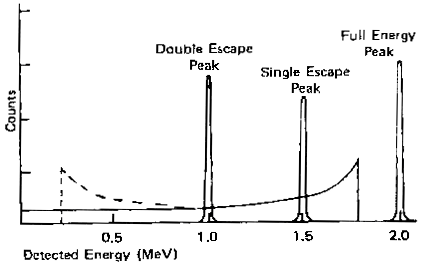
\includegraphics[width= 0.75 \linewidth]{charts/Spektrumschema}
				\caption{
					Schematische Darstellung des Compton-Effekts.
					\cite{Anleitung}
				}
				\label{fig_Gammaspektrum}
		\end{figure}

	\subsection{Gamma-Detektoren}

	\subsubsection{Halbleiterdetektoren}
	%TODO pn-Übergang? als gamma-detektor?
	%TODO Problem herstellung von "pure semiconductor"
	%TODO Was ist wichtig bei Verwendung von Halbleiterdetektor?
	%TODO Warum muss der gekühlt werden?
	%TODO Was braucht man sonst noch?
	%TODO Warum Schicht undotierte Schicht?-> breitere RLZ
	%TODO Unterschiede Szintallator und Halbleiter

	Der Übergang zwischen p- und n-dotiertem Halbleiter wird als pn-Übergang bezeichnet.
	Durch die überschüssigen bzw. fehlenden Elektronen im Gitter und den folgenden Ladungsfluss, bei dem Elektronen und Löcher rekombinieren, entsteht im pn-Übergang eine Raumladungszone.
	Diese ist räumlich begrenzt, da der Rekombination das Coulombfeld der verschobenen Ladungen gegenübersteht.

	Wenn ein Photon auf das Halbleitermaterial trifft, entsteht ein Elektron-Loch-Paar.
	Elektron und Loch können sich durch den Halbleiter bewegen und, wenn sie sich treffen, rekombinieren.
	Wenn sie jedoch durch das elektrische Feld der Raumladungszone (das durch eine äußere Hochspannung vergrößert wird) getrennt und nachgewiesen werden.


	\subsubsection{Szintallationsdetektor} % (von woanders klaubar)
	%TODO welche gibt es, was sind die Unterschiede?
	%TODO warum dotiert?
	%TODO Photomultiplier? Was braucht man da sonst noch?->Lichtleiter, Vorverstärker.
	%TODO Auswahlkriterien für Szintallator für Gamma-Spektroskopie

	\subsubsection{Kalibrierung}
	%TODO Warum Na-22 zur Kalibrierung?
	%TODO wie beeinflusst die Kalibrierunsicherheit die späteren Messungen?
	%TODO Was bestimmt Peakbreite?
	%TODO Warum misst man die Breite?
	%TODO Definition FWHM, Sigma
	%TODO kann man hier Kalibrierunsicherheit vernachlässigen?

	\section{Methoden}
	% Bilder von der Website klauen
	% einer will Präsens
	%TODO verwendete Proben
	%TODO Wahl des Verstärkungsfaktors (pro Detektor gleich gelassen) -> so, dass alle Peaks im Spektrum sind durch kurzzeitmessung
	%TODO Messdauern?
	%TODO Erzprobe

	\section{Ergebnisse und Diskussion}
	%TODO Unsicherheiten


	\subsection{Beobachtung und Datenanalyse}
	% Allgemeine Beobachtungen
	% Einflüsse von veränderten Parametern auf Messung

	\subsubsection{Unsicherheiten}
	Alle Unsicherheiten werden nach GUM bestimmt und berechnet.
	Für diese Berechnungen wurde die Python Bibliothek \enquote{uncertainties} herangezogen, welche den Richtlinien des GUM folgt.
	Die Fits verwenden die Methode der kleinsten Quadrate, außer wenn anders angegeben.
	Die Unsicherheit der gemessenen Ereignisse $N$ ist durch $\sqrt{N}$ gemäß Poisson-Verteilung gegeben.
	\subsubsection{Modell}
	Die aufgenommenen Spektren der $^{22}$Na-Probe sind in \cref{fg_Na_ch} abgebildet.
	Es wurden bei jeder Messung die ersten 95 Kanäle vernachlässigt, da all diese nahe Null Ereignisse liefern und die Erstellung ein physikalischen Modells des Spektrums im Randbereich unmöglich machen. %TODO schönerer Satz wäre schöner
	Das Modell wurde in \enquote{Fityk} aus Gaußkurven zusammengesetzt.
	\begin{figure}[H]
		\centering
		\begin{subfigure}[c]{\textwidth}
			\centering
			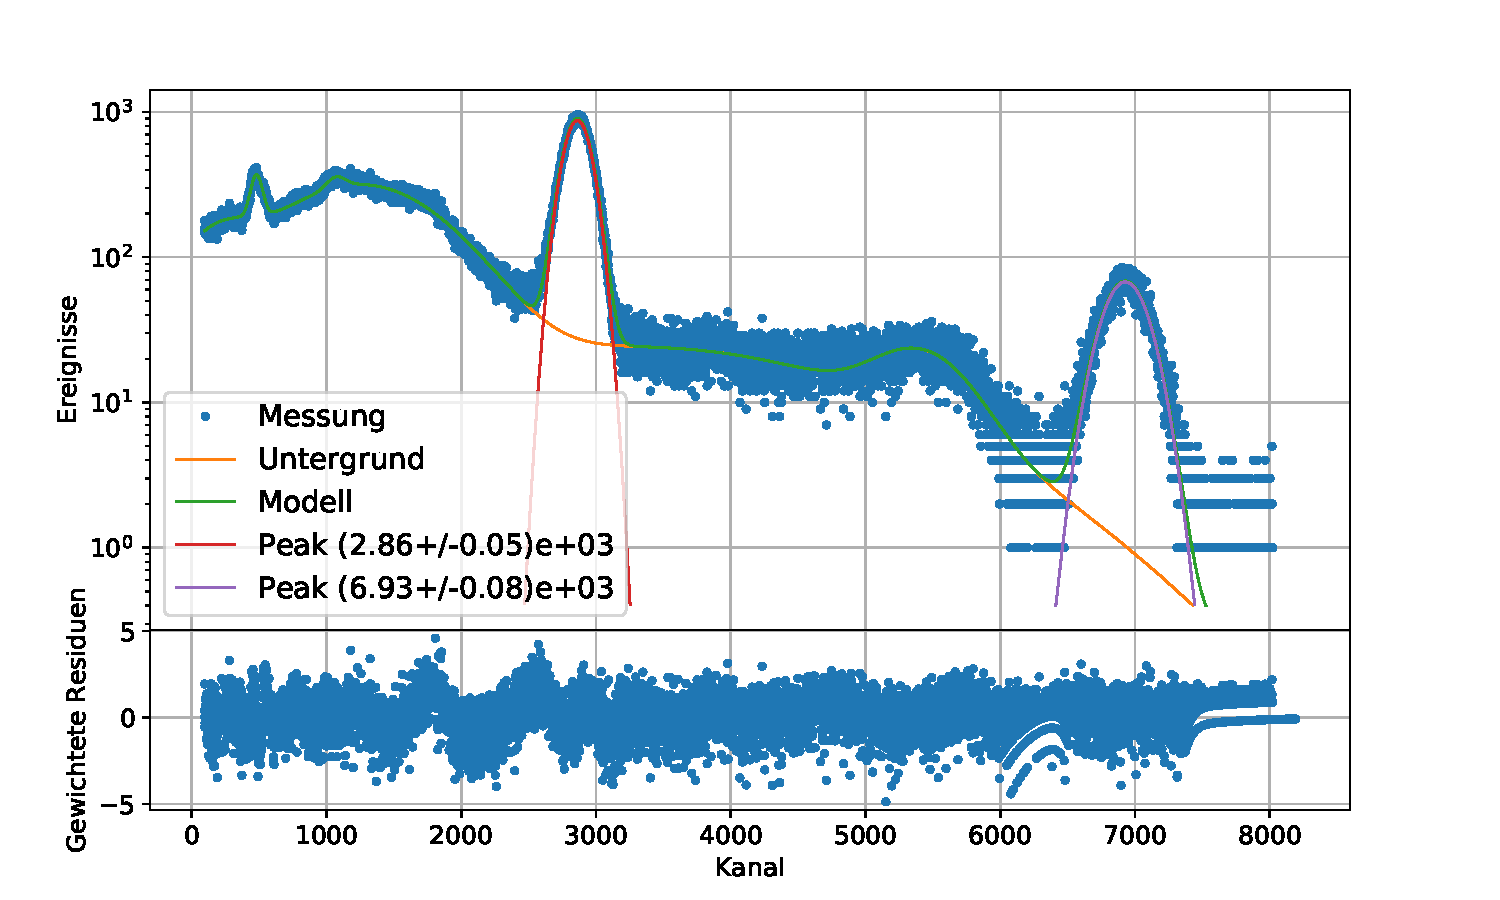
\includegraphics[width= 1 \linewidth]{img/NaNaCh.pdf}
			\subcaption{
				NaI-Detektor.
			}
		\end{subfigure}
		\begin{subfigure}[c]{\textwidth}
			\centering
			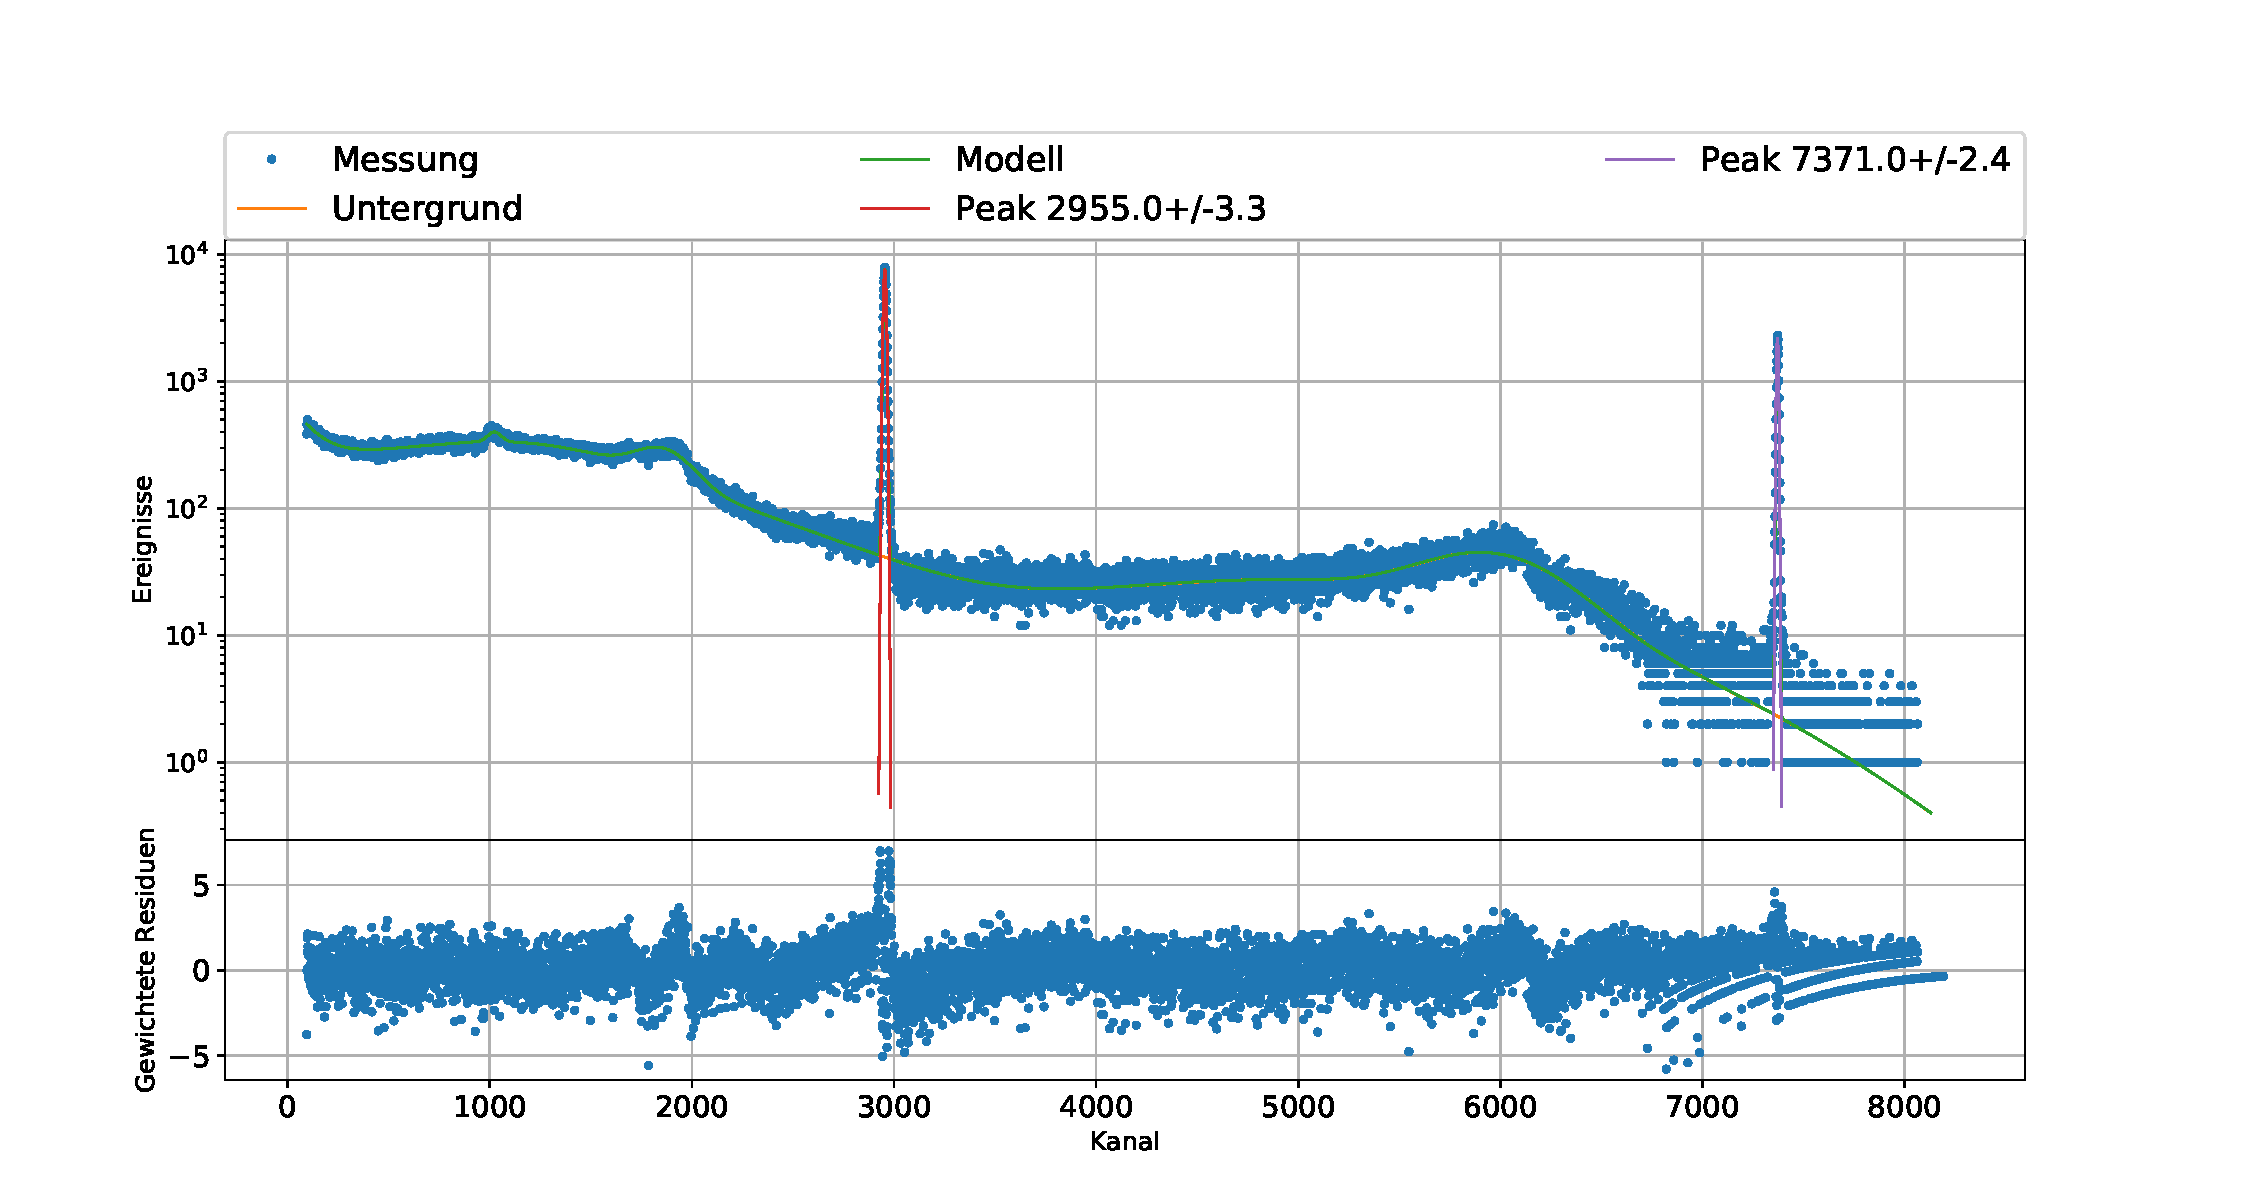
\includegraphics[width= 1 \linewidth]{img/NaGeCh.pdf}
			\subcaption{
				Ge-Detektor.
			}
		\end{subfigure}
		\caption{$^{22}$Na-Probe}
		\label{fg_Na_ch}
	\end{figure}


	\subsubsection{Kalibration}
  Mittels der Literaturwerte der Peaks der $^{22}$Na-Probe (\SI{511}{keV} und \SI{1274}{keV} \cite{Anleitung}) lassen sich die Kanäle umrechnen zu einer Energieskala.  %TODO erläutert in Theorie?
	In \cref{fg_kali_mix} sind in blau (gelb) die zwei Kalibrationspunkte für den NaI-Detektor (Ge-Detektor) abgebildet.
	Die Unsicherheit des Kanals ist durch die Standardunsicherheit der Gaußkurve in \cref{fg_Na_ch} gegeben.

	\begin{figure}[H]
			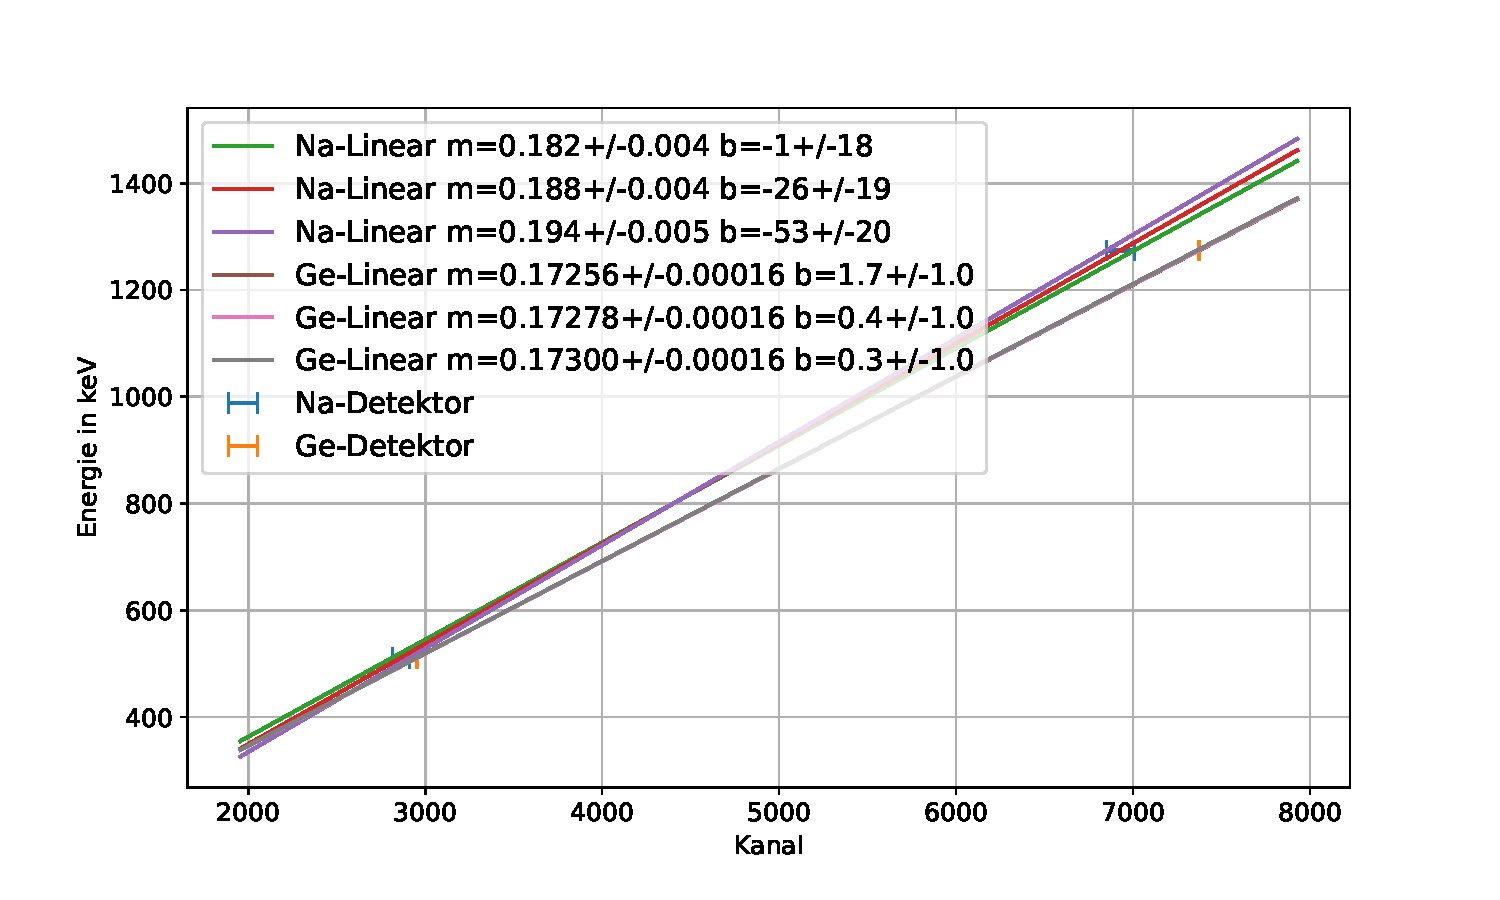
\includegraphics[width= 0.8 \linewidth]{img/kali_mix.pdf}
			\caption{
				Kalibrationsgeraden $f(x)=mx+b$.
				$m$ ist die Steigung der Gerade in \si{keV}.
				$b$ ist der y-Achsenabschnitt in \si{keV}.
			}
			\label{fg_kali_mix}
	\end{figure}

	Da ein linearer Fit zwischen zwei Punkten mit Unsicherheiten mit dem \enquote{Least-Square-Fit} nicht zielführend ist, werden drei Geraden durch die Messintervalle gelegt, sodass sich eine mittlere, maximale und minimale Steigung ergeben. %TODO hier wird er wissen wollen, warum der nicht zielführend ist.
	Eine Mittelung dieser Werte ist in \cref{tb_kali_avg} aufgeführt.

\begin{table}[H]
		\centering
		\begin{tabular}{c | c | c  }
			 Detektor& $m$ in \si{kev}& $b$ in \si{keV} \\ \hline
			 NaI & \SI{0.188+-0.015}{} & \SI{-30+-60}{} \\
			 Ge & \SI{0.1728+-0.0006}{} & \SI{1.3+-2.3}{} \\
		\end{tabular}
		\caption{
		Gemittelte Kalibrationsparameter für NaJ- und Ge-Detektor.
		}
		\label{tb_kali_avg}
\end{table}
%TODO y-Achse ist ca. Null, nice, aber diskutieren warum Anfang alles Null?
Damit lässt sich ein Kanal $c$ nach \cref{eq_trans} in die Energie $E$ transformieren.
\begin{equation}
	\label{eq_trans}
	E = m\cdot c + b
\end{equation}

\subsection{Peaks und Kanten}
In \crefrange{fg_Na}{fg_Mix} sind die kalibrierten Spektren von vier Proben für jeden der Detektoren dargestellt.
Die horizontalen Linien, die sich im höher energetischen Bereich ergeben, entstehen durch die logarithmischen Darstellung.

%TODO In der Theorie?
Die Comptonkante berechnet sich aus dem Literaturwert:
\begin{equation}
	E_c = E_\gamma - \frac{E_\gamma }{1+2E_\gamma/m_ec^2}
\end{equation}
Die Rückstreukante ist analog:
\begin{equation}
	E_c =  \frac{E_\gamma}{1+E_\gamma/m_ec^2}
\end{equation}
Die Literaturwert stammen aus \cite{Anleitung}.
Außerdem wurden die Ränder des Bereichs der Röntgenfluoreszenz von Blei gekennzeichnet (aus \cite{XRAYDB}).


%TODO caption ? Unsicherheit?
\begin{figure}[H]
		\centering
		\begin{subfigure}[c]{\textwidth}
			\centering
			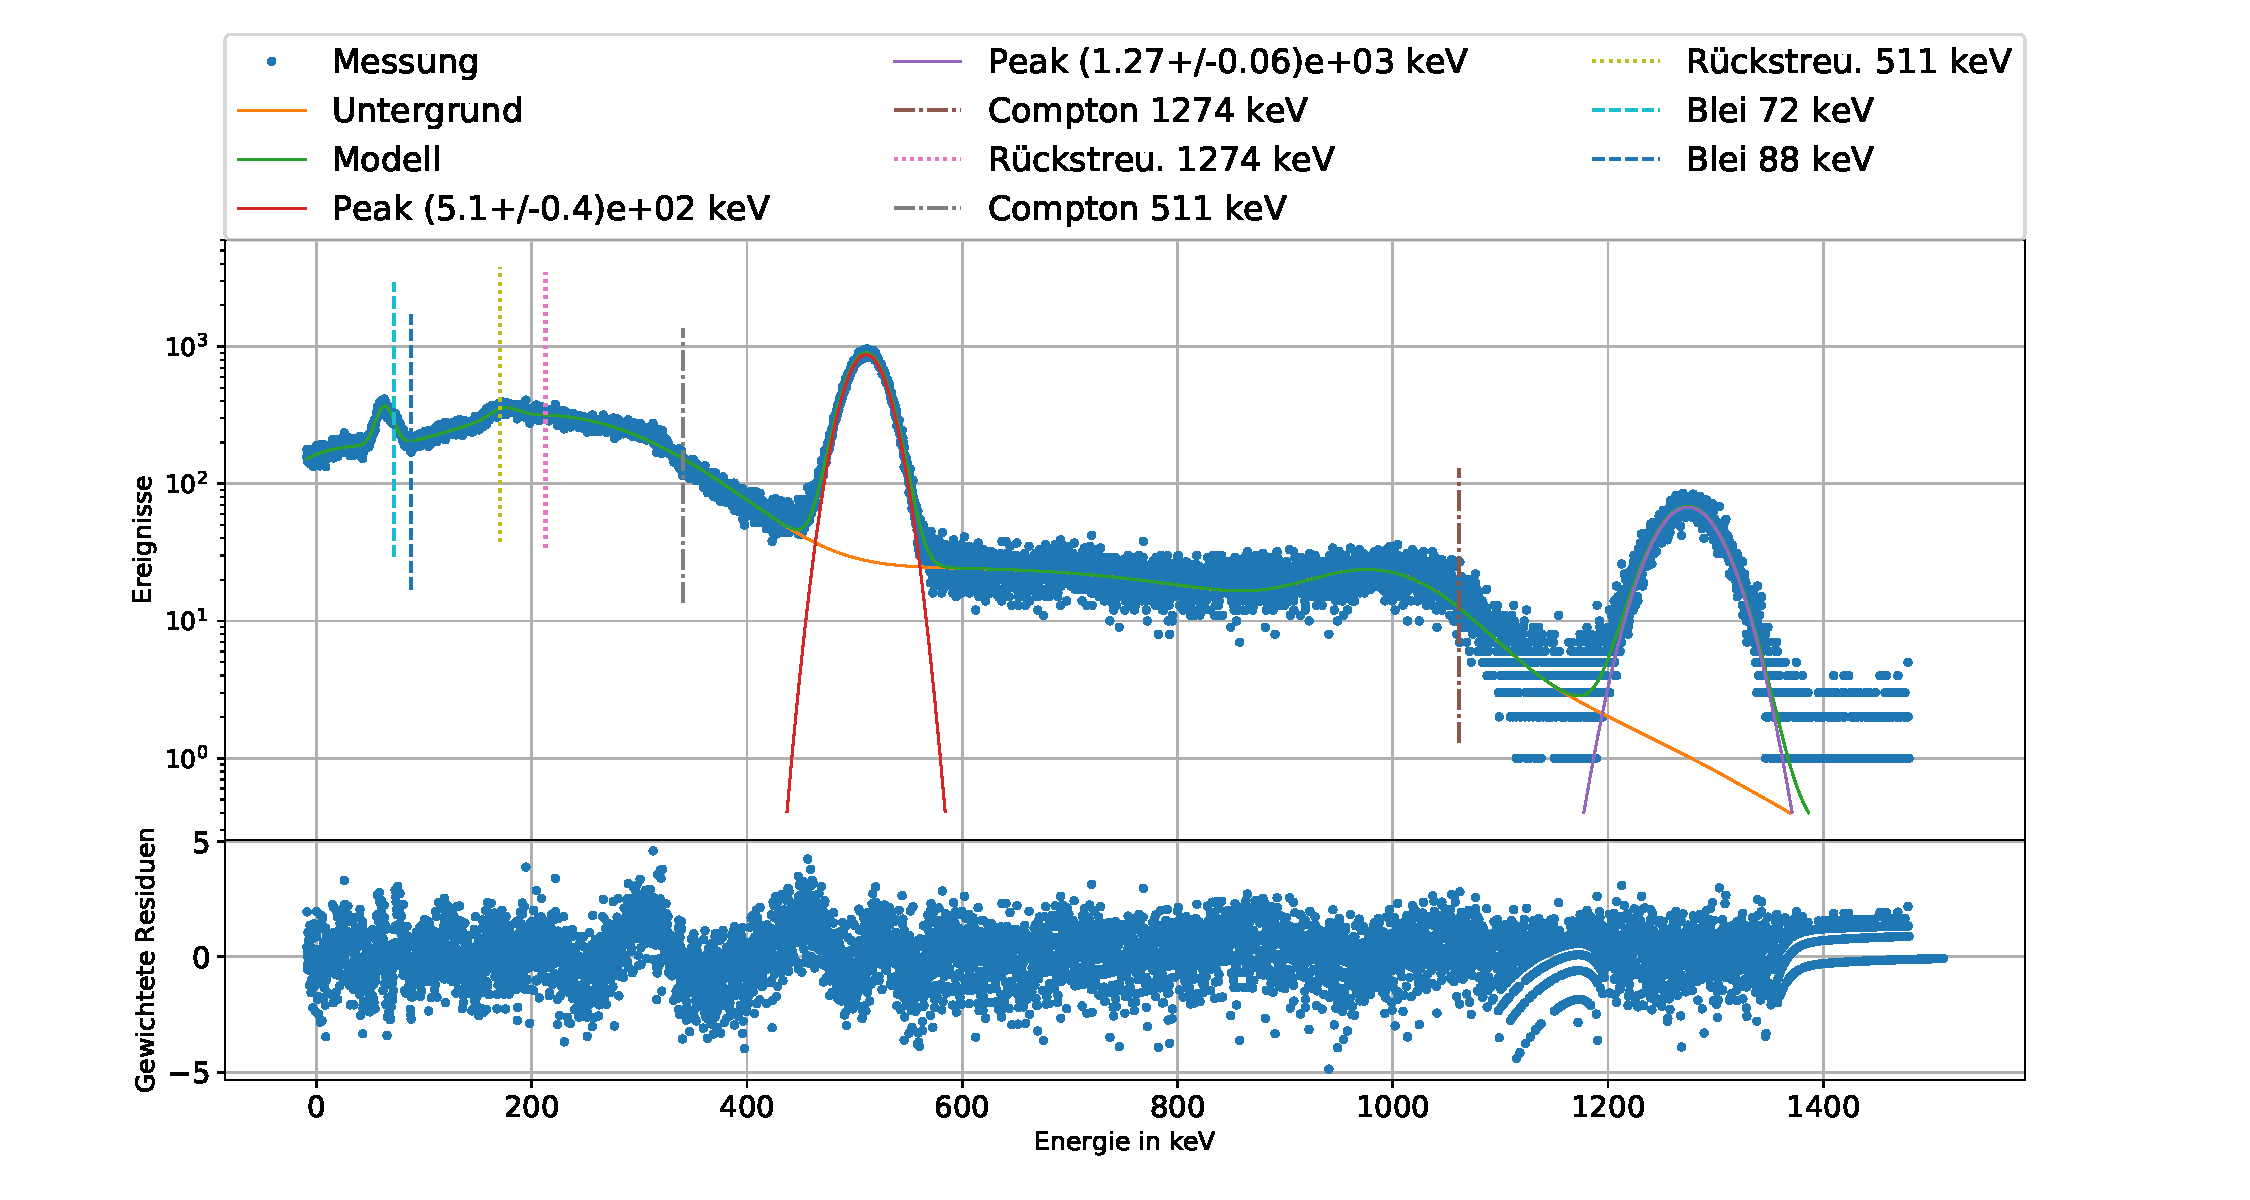
\includegraphics[width= 1 \linewidth]{img/NaNa.pdf}
			\subcaption{
				NaI-Detektor.
			}
		\end{subfigure}
		\begin{subfigure}[c]{\textwidth}
			\centering
			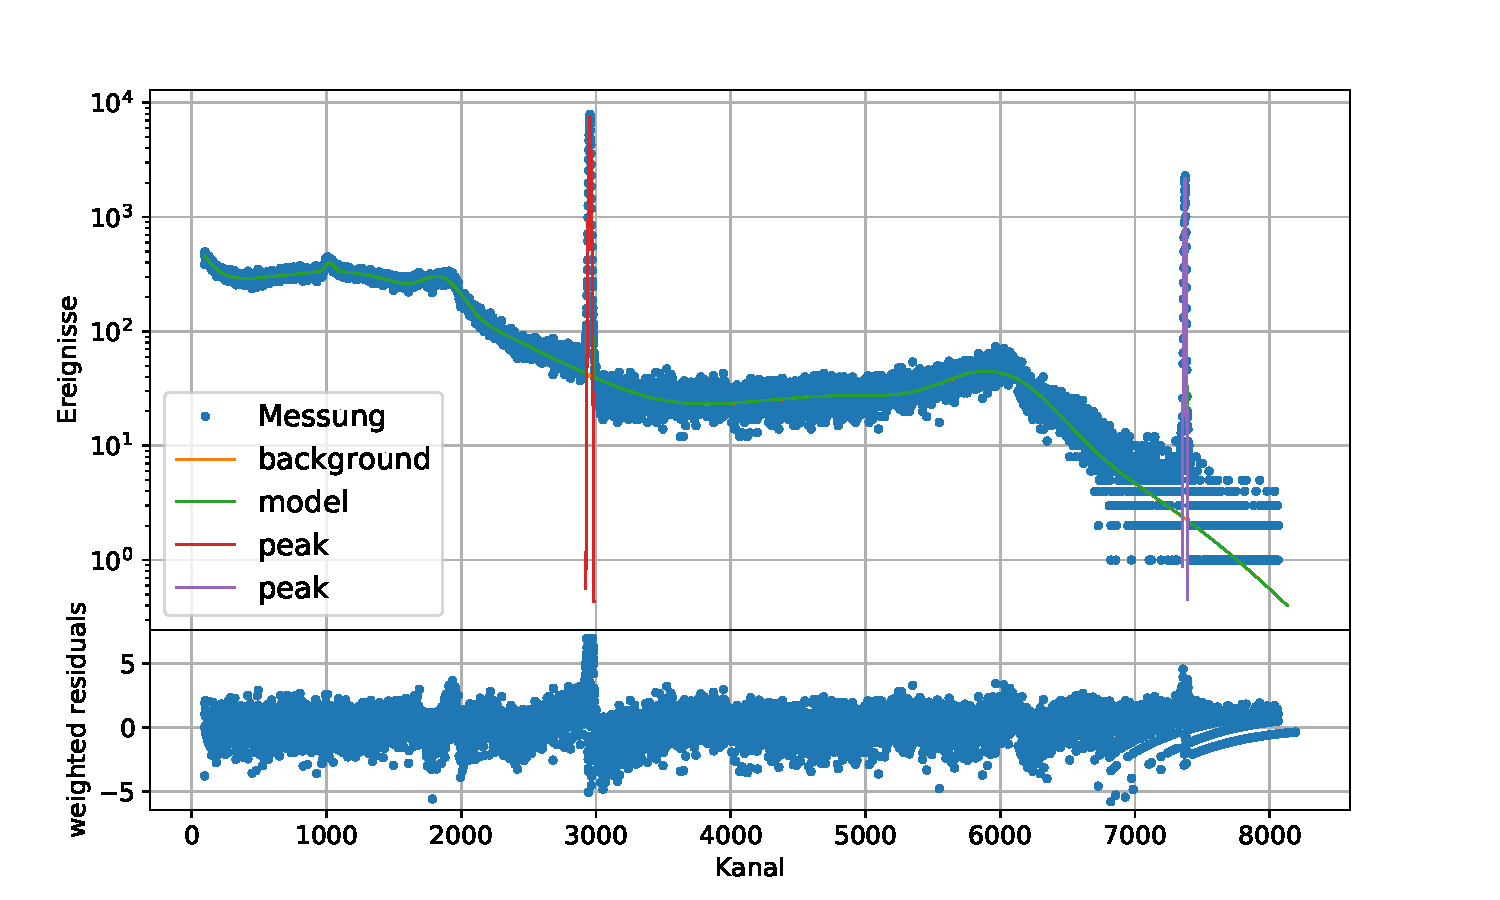
\includegraphics[width= 1 \linewidth]{img/NaGe.pdf}
			\subcaption{
				Ge-Detektor.
			}
		\end{subfigure}
		\caption{$^{22}$Na-Probe}
		\label{fg_Na}
	\end{figure}


\begin{figure}[H]
		\centering
		\begin{subfigure}[c]{\textwidth}
			\centering
			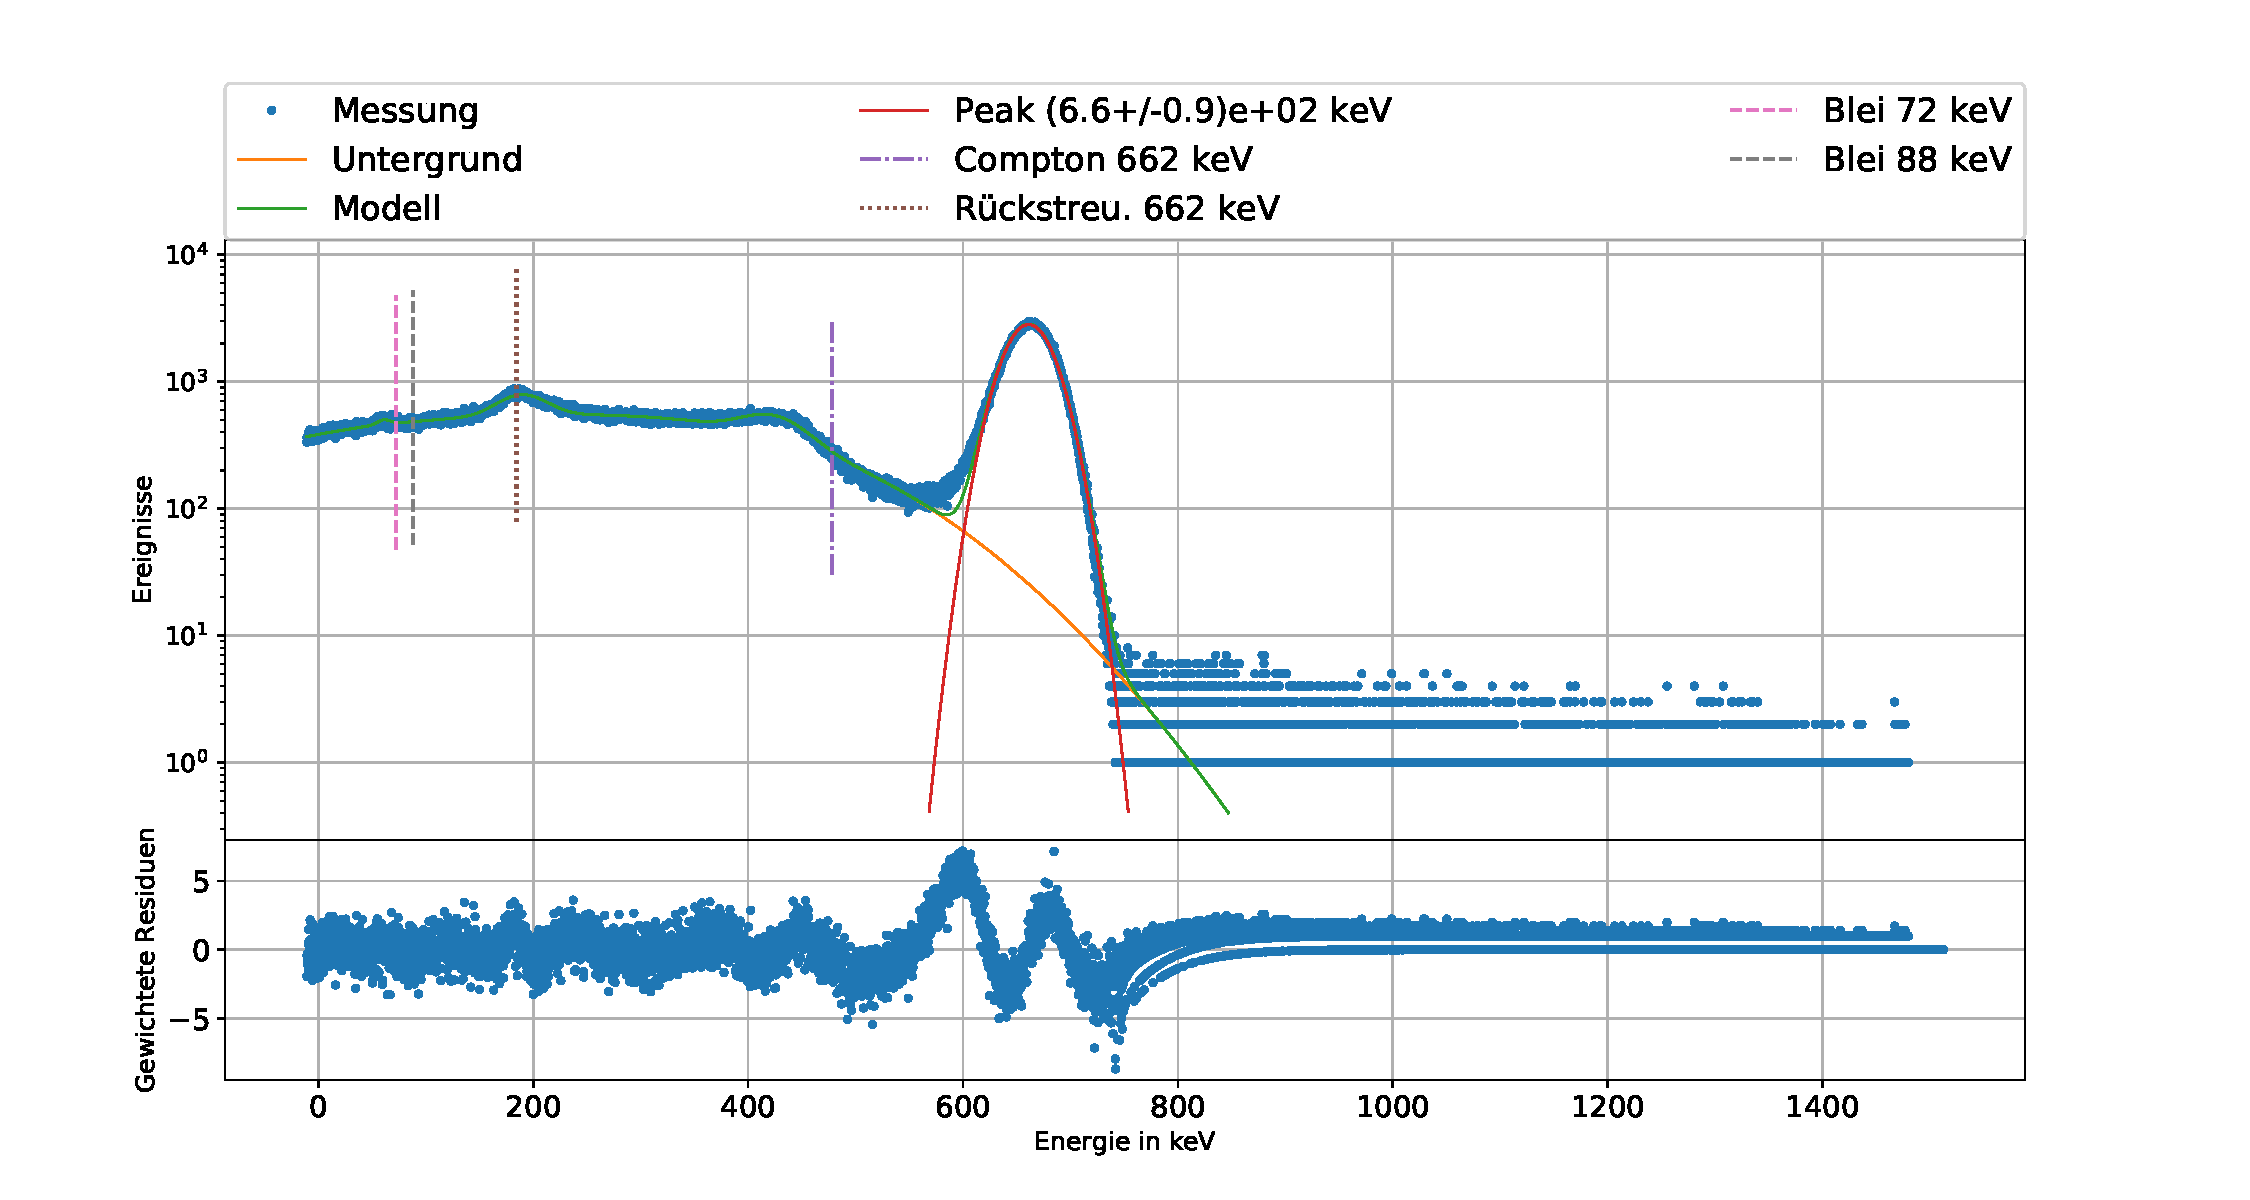
\includegraphics[width= 1 \linewidth]{img/CsNa.pdf}
			\subcaption{
				NaI-Detektor.
			}
		\end{subfigure}
		\begin{subfigure}[c]{\textwidth}
			\centering
			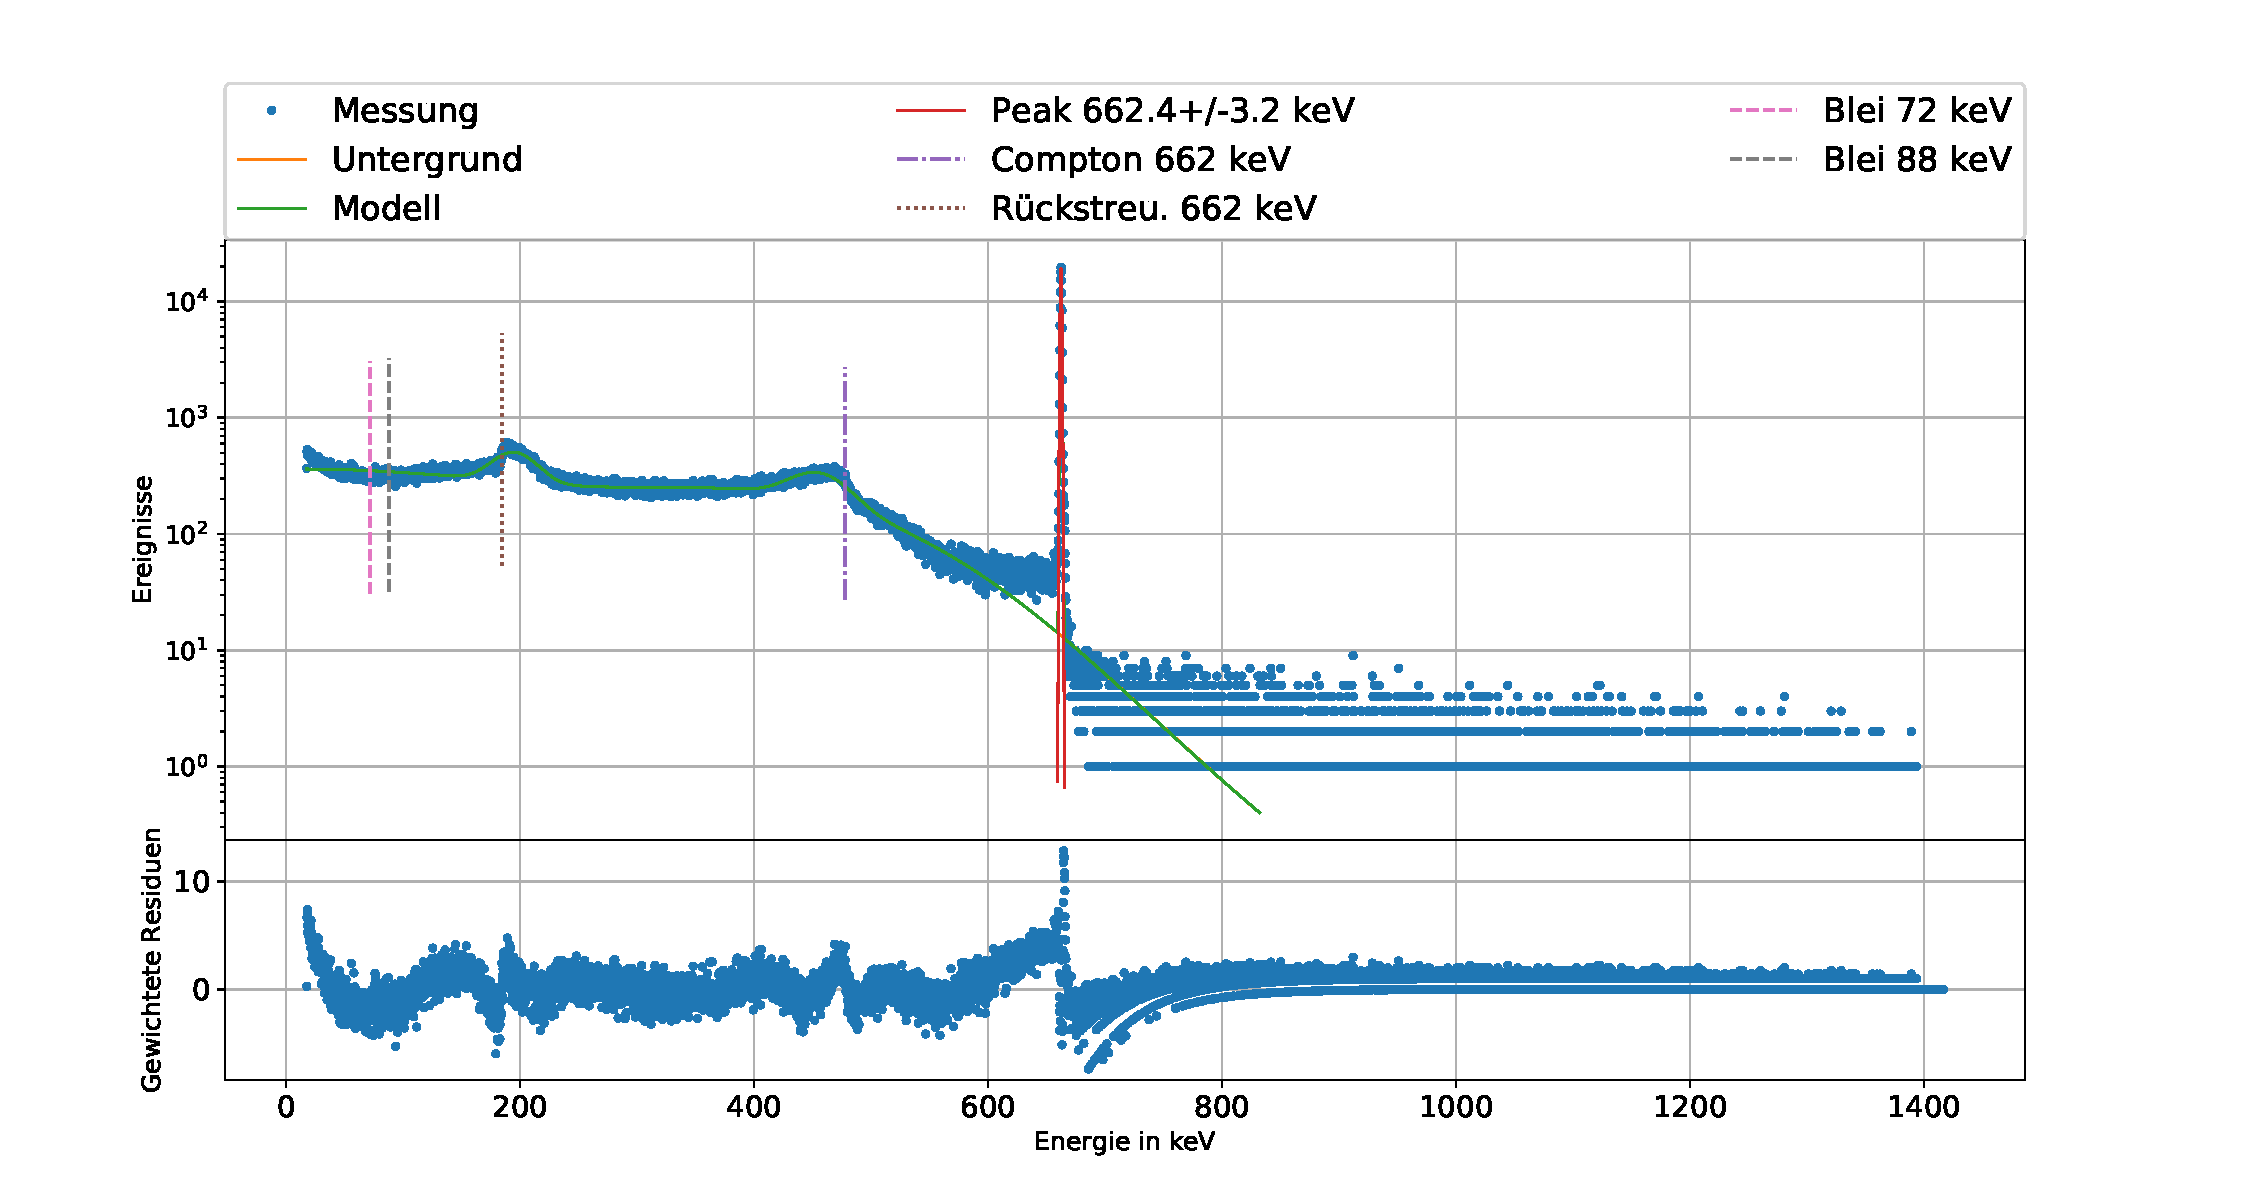
\includegraphics[width= 1 \linewidth]{img/CsGe.pdf}
			\subcaption{
				Ge-Detektor.
			}
		\end{subfigure}
		\caption{$^{137}$Cs-Probe}
		\label{fg_Cs}
	\end{figure}

\begin{figure}[H]
		\centering
		\begin{subfigure}[c]{\textwidth}
			\centering
			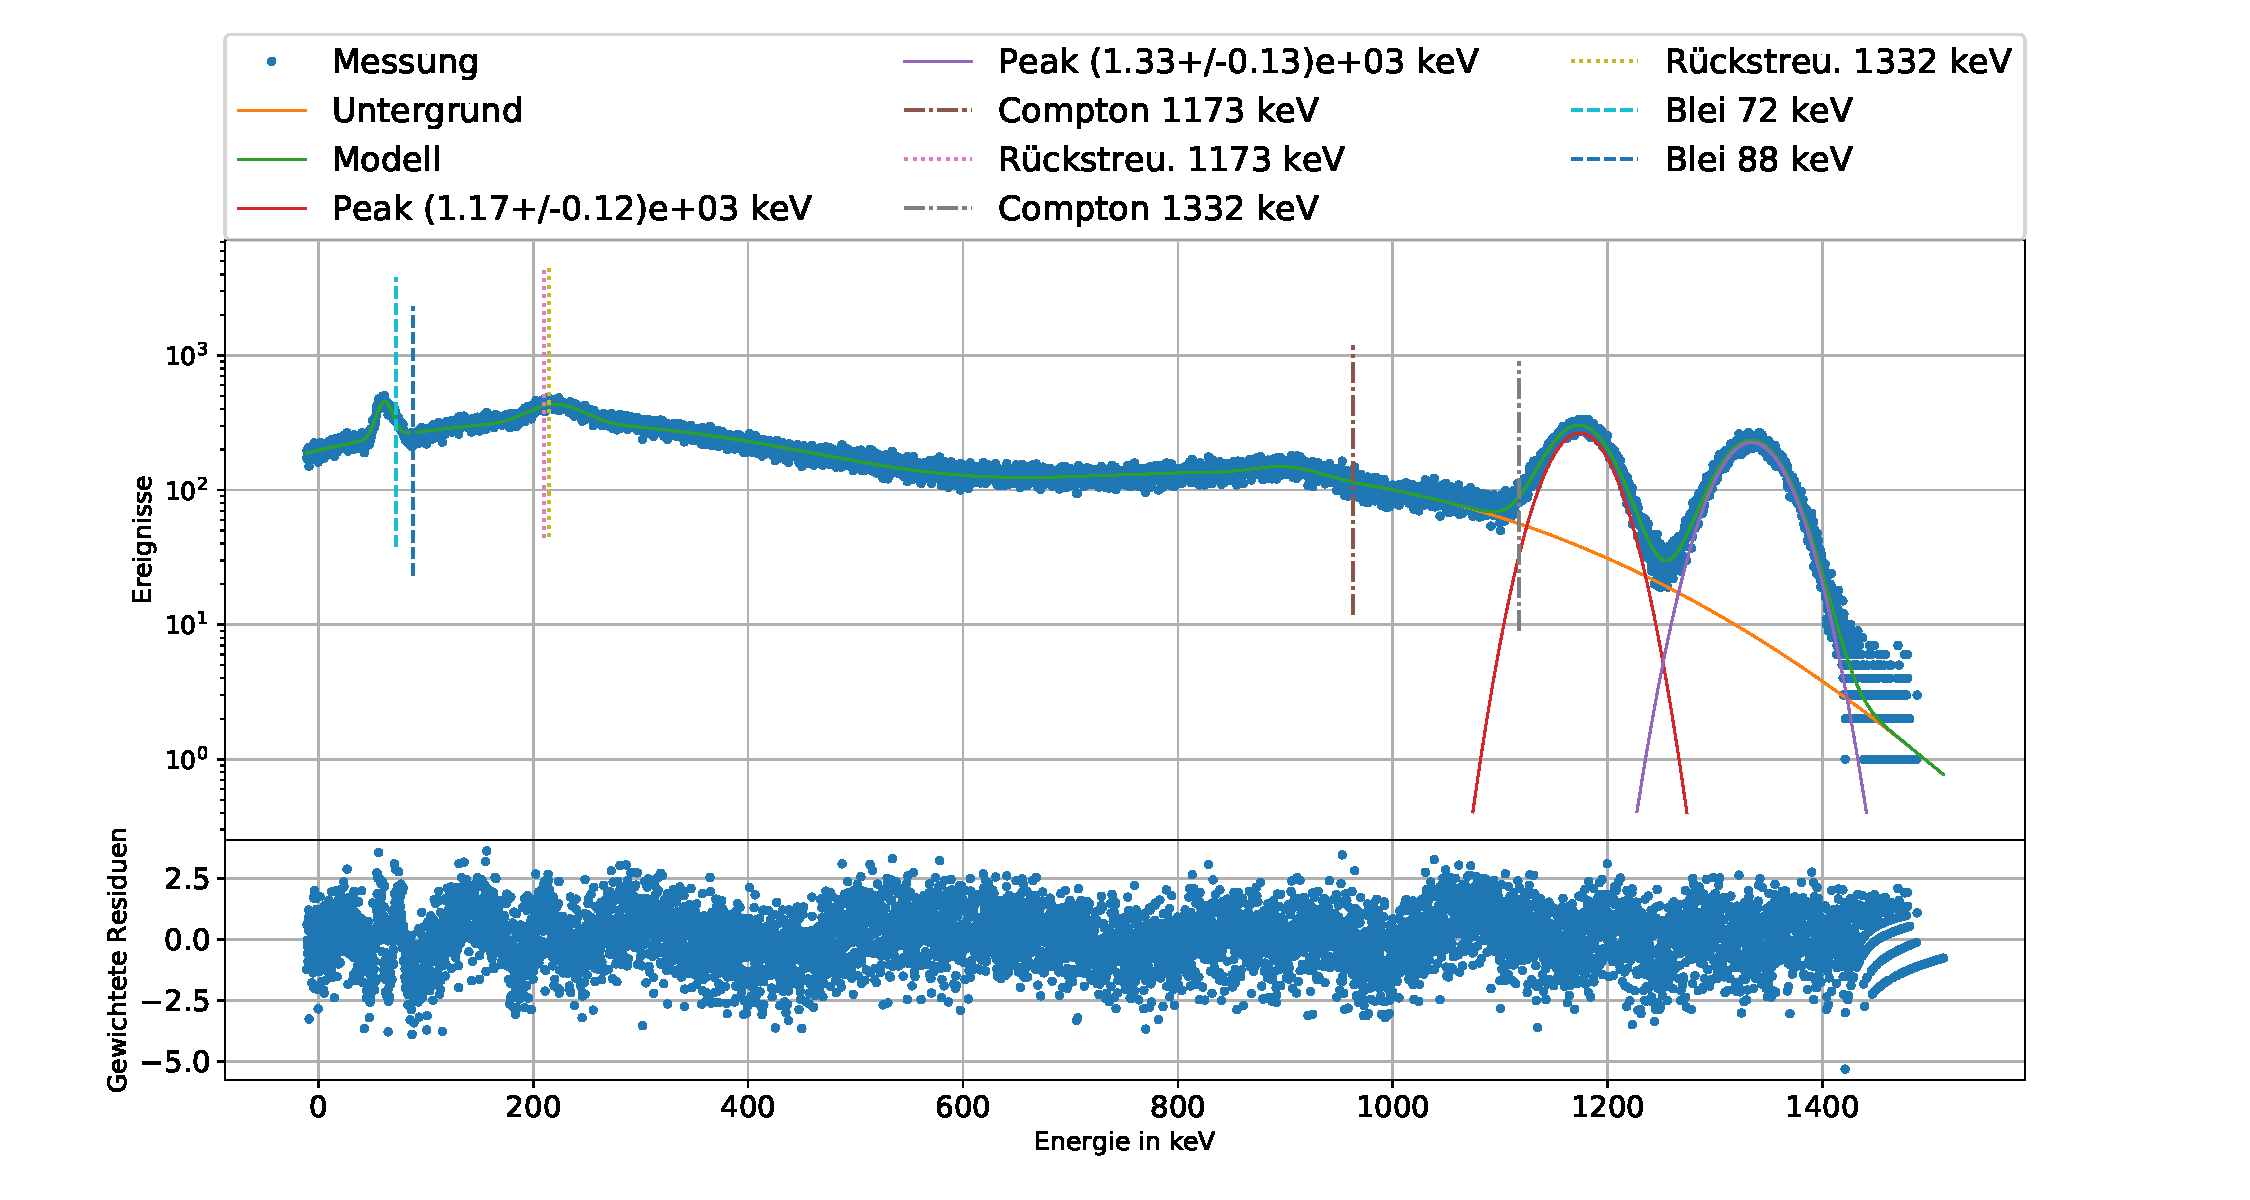
\includegraphics[width= 1 \linewidth]{img/CoNa.pdf}
			\subcaption{
				NaI-Detektor.
			}
		\end{subfigure}
		\begin{subfigure}[c]{\textwidth}
			\centering
			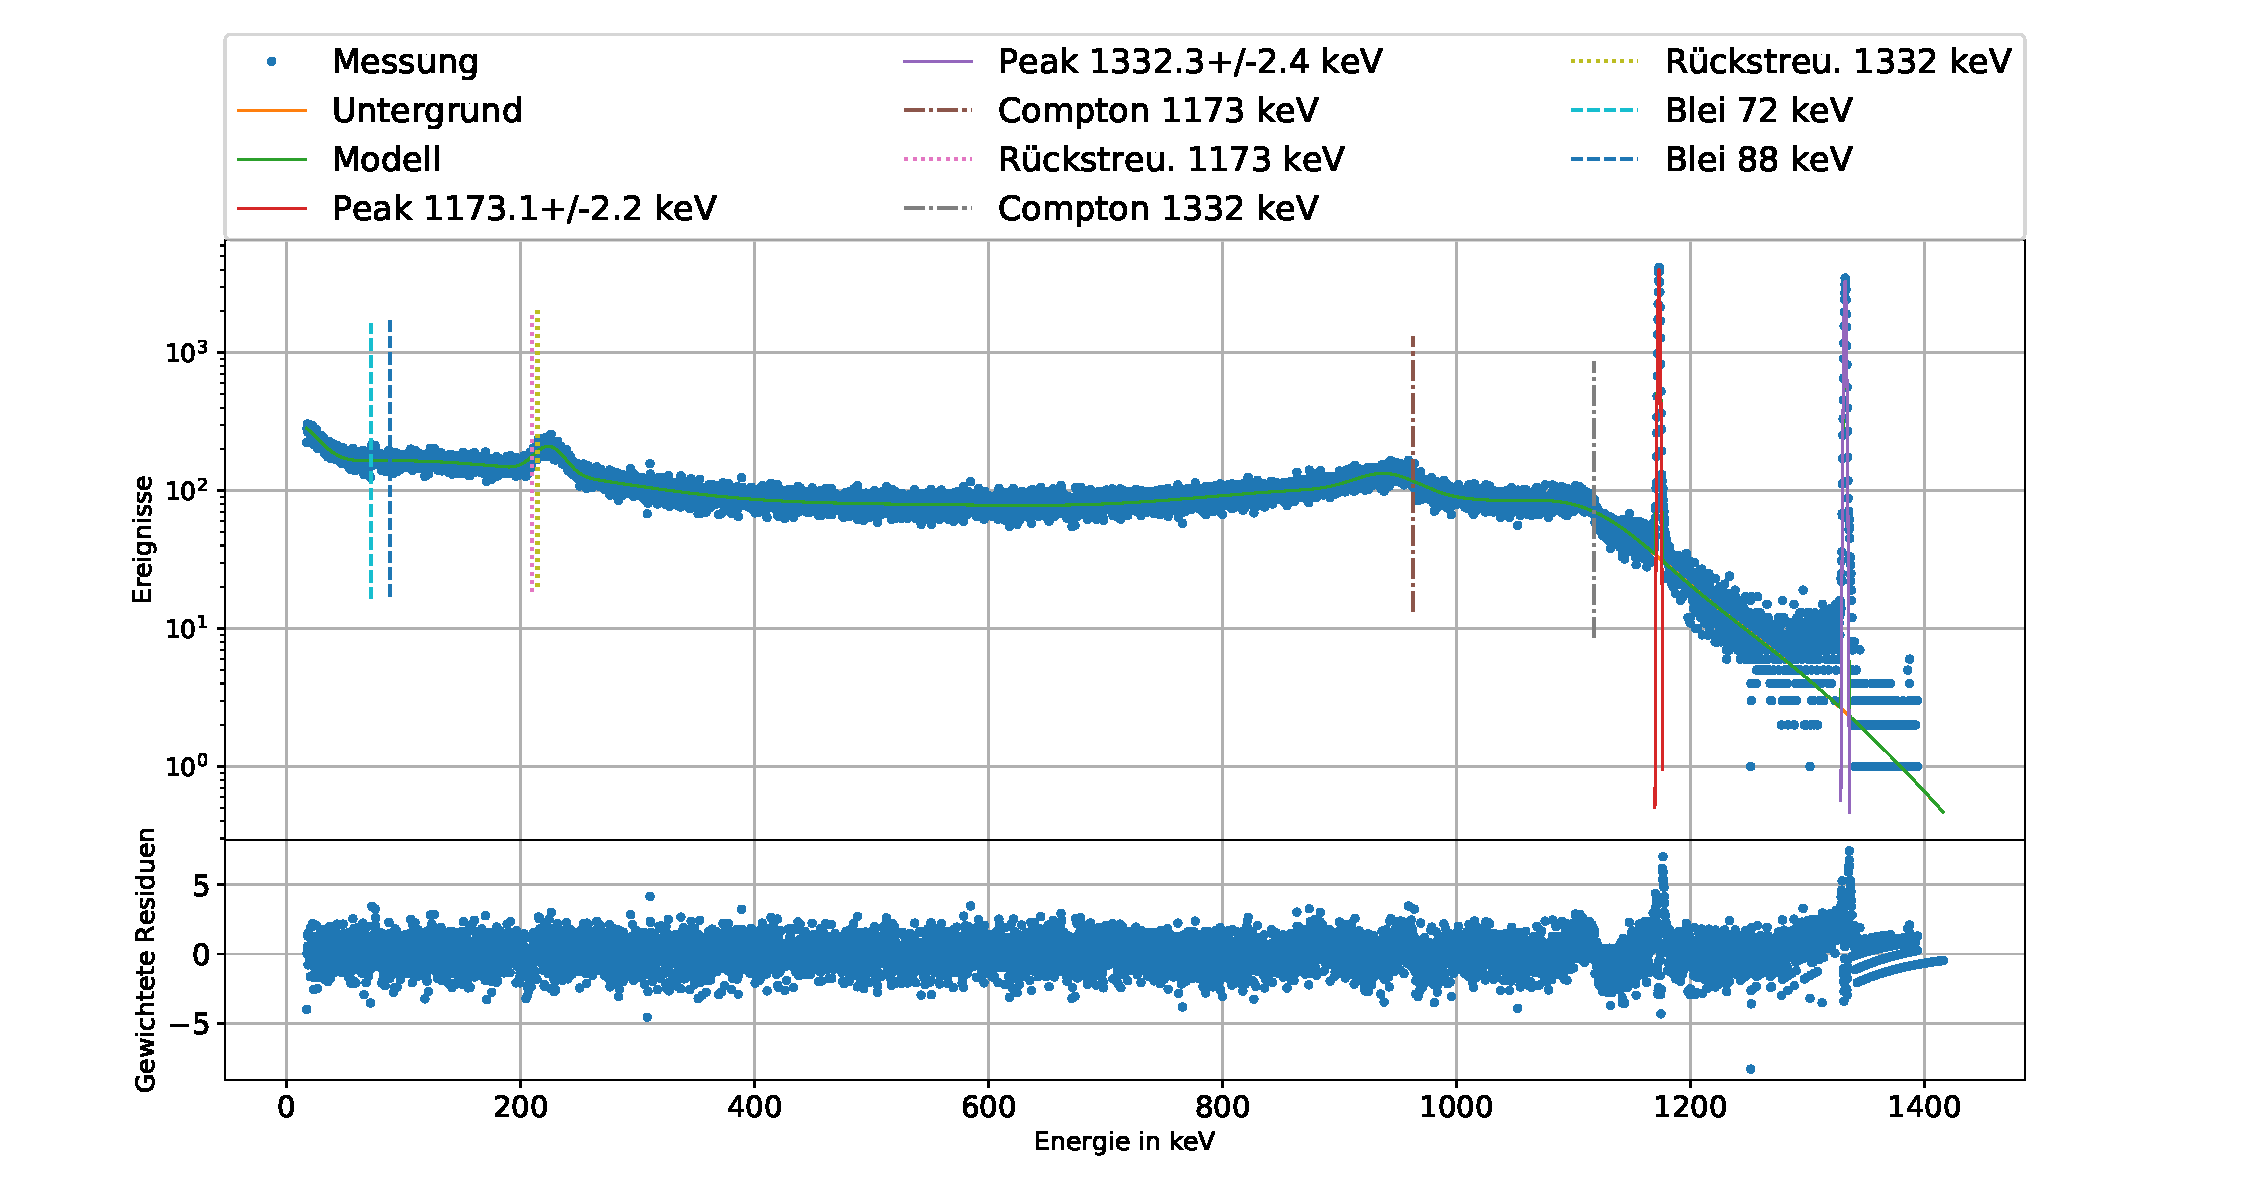
\includegraphics[width= 1 \linewidth]{img/CoGe.pdf}
			\subcaption{
				Ge-Detektor.
			}
		\end{subfigure}
		\caption{$^{57}$Co-Probe}
		\label{fg_Na}
	\end{figure}

\begin{figure}[H]
		\centering
		\begin{subfigure}[c]{\textwidth}
			\centering
			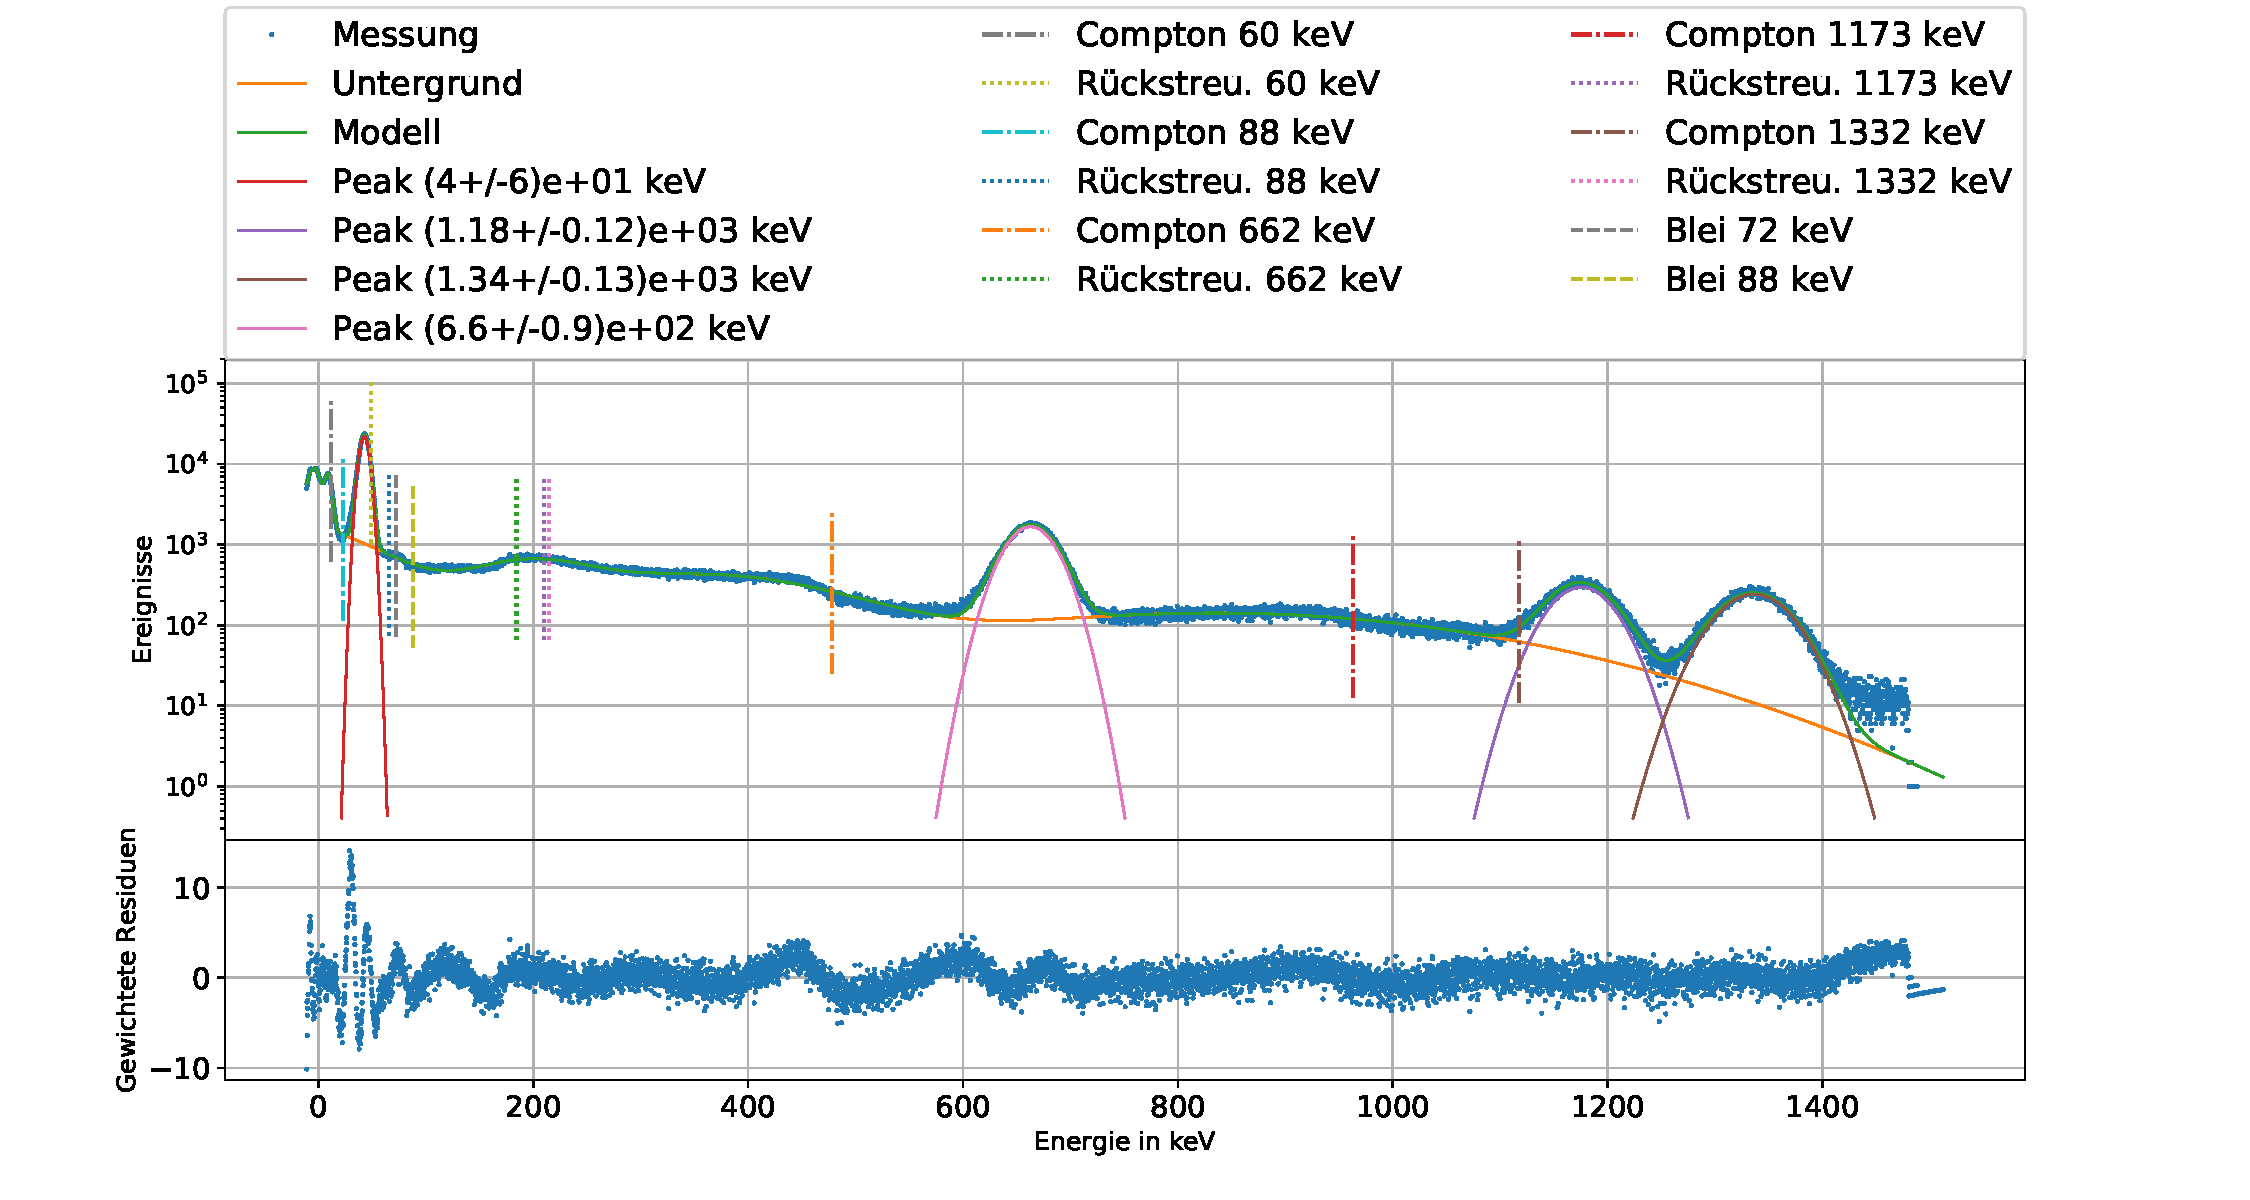
\includegraphics[width= 1 \linewidth]{img/MixNa.pdf}
			\subcaption{
				NaI-Detektor.
			}
		\label{fg_Mix_Na}
		\end{subfigure}
		\begin{subfigure}[c]{\textwidth}
			\centering
			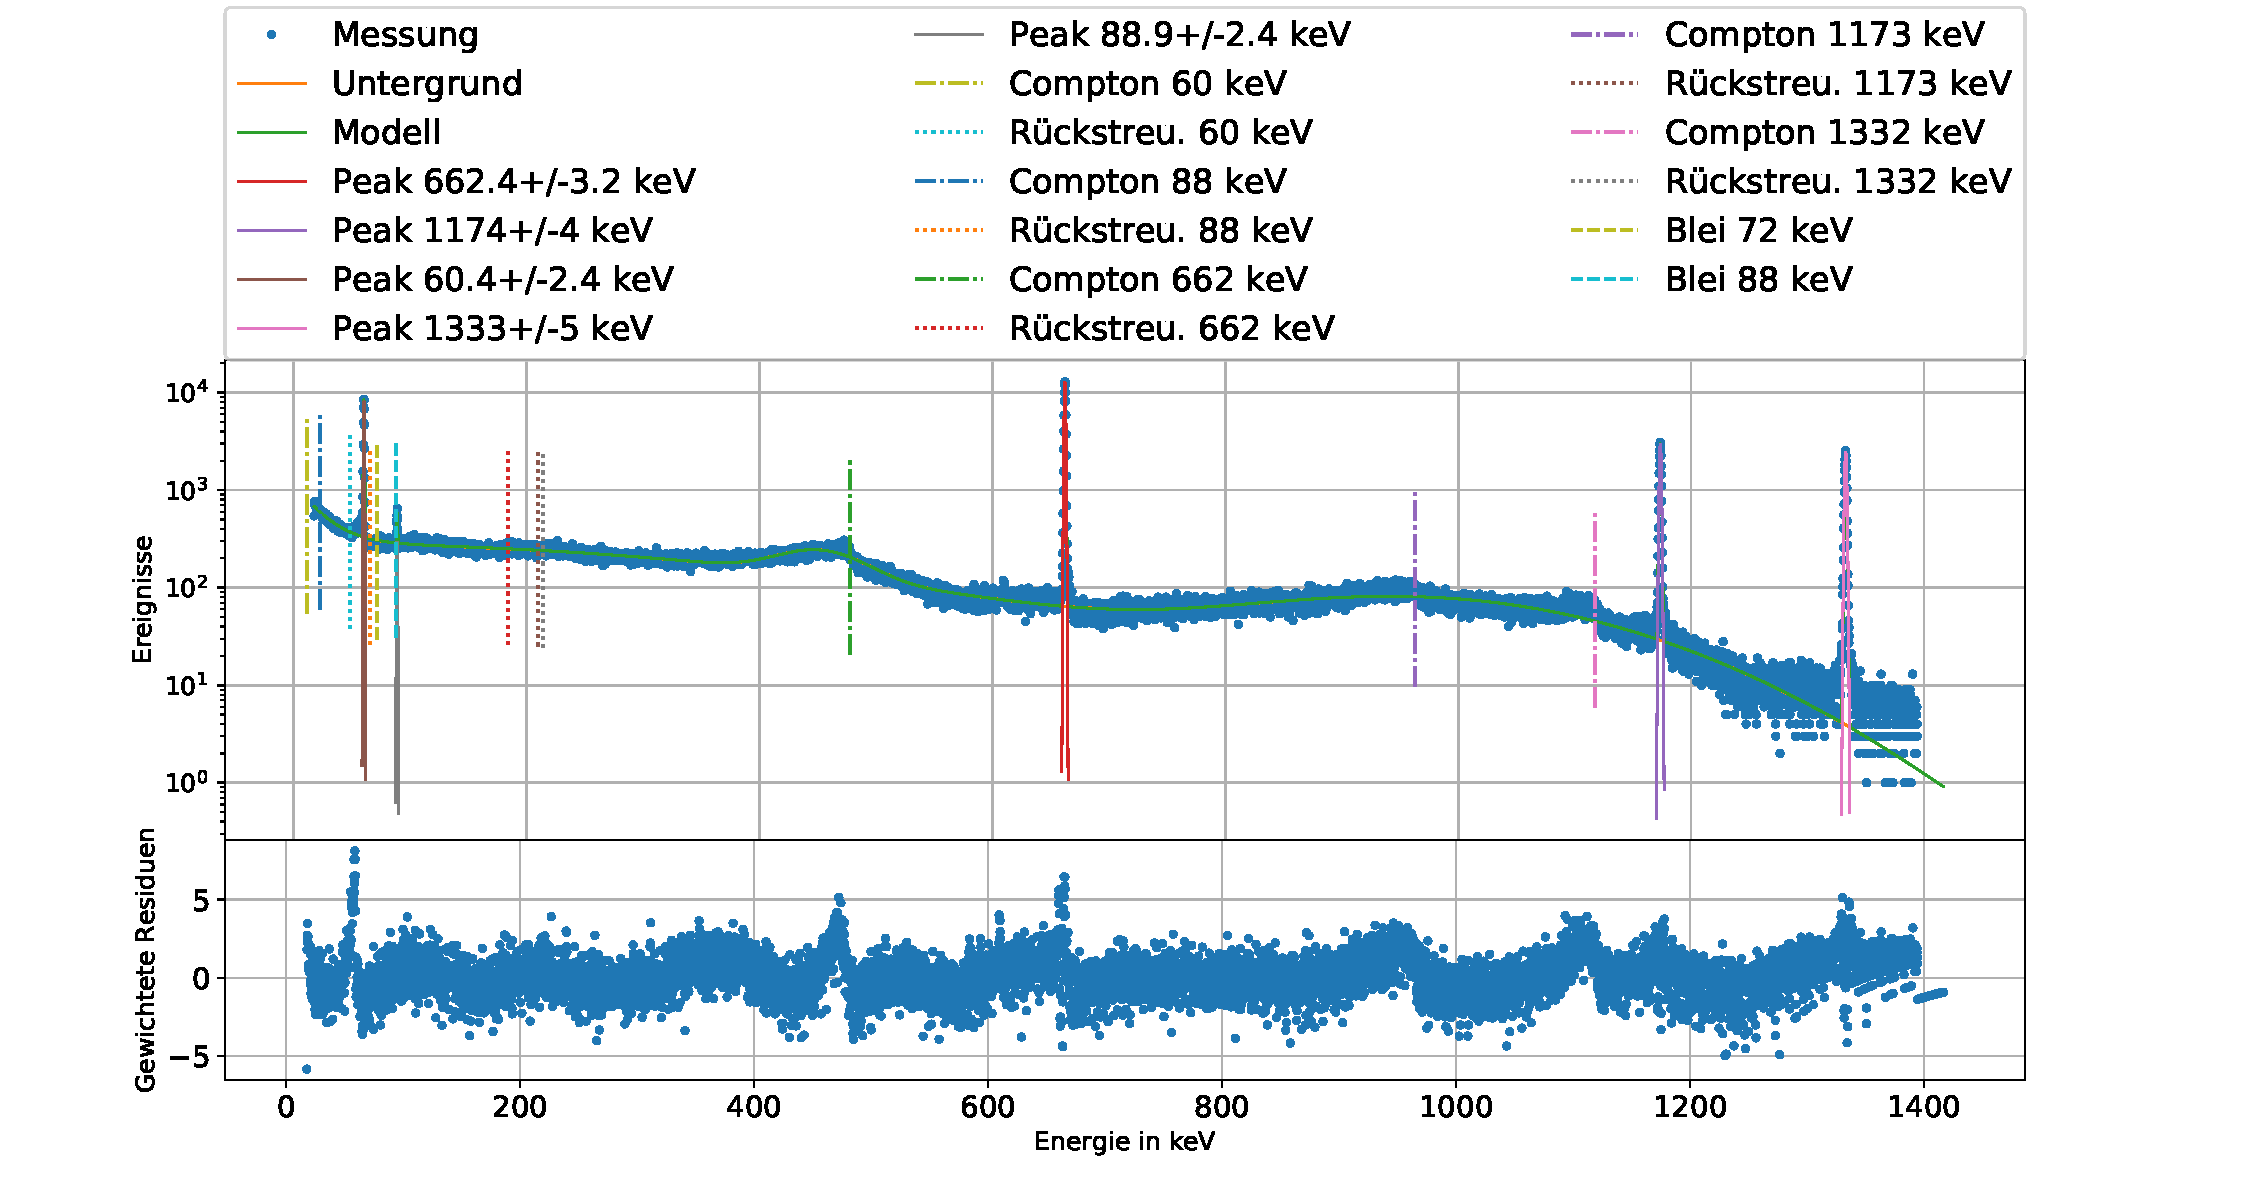
\includegraphics[width= 1 \linewidth]{img/MixGe.pdf}
			\subcaption{
				Ge-Detektor.
			}
		\label{fg_Mix_Ge}
		\end{subfigure}
		\caption{Misch-Probe}
		\label{fg_Mix}
	\end{figure}


\subsection{Nichtlinearität des Detektors}
Die Nichtlinearität des Detektors kann gezeigt werden, indem man die relative Differenz der gemessenen Peaks gegen den Referenzwert des Peaks aufträgt.
Also
\begin{equation}
	\delta(E_r) = 1- \frac{E_m}{E_r}
\end{equation}
Diese Differenz wurde  in \cref{fg_diff_na} und \cref{fg_diff_ge} für NaI- und Ge-Detektor dargestellt.
$E_r$ ist Literaturwert (aus \cref{fig_zerfallsschemata}) für die Peakposition und $E_m$ ist der gemessenen Wert.

%TODO log plot hier von?
%TODO no errors hier?
\begin{figure}[H]
		\centering
		\begin{subfigure}[t]{0.8\textwidth}
			\centering
			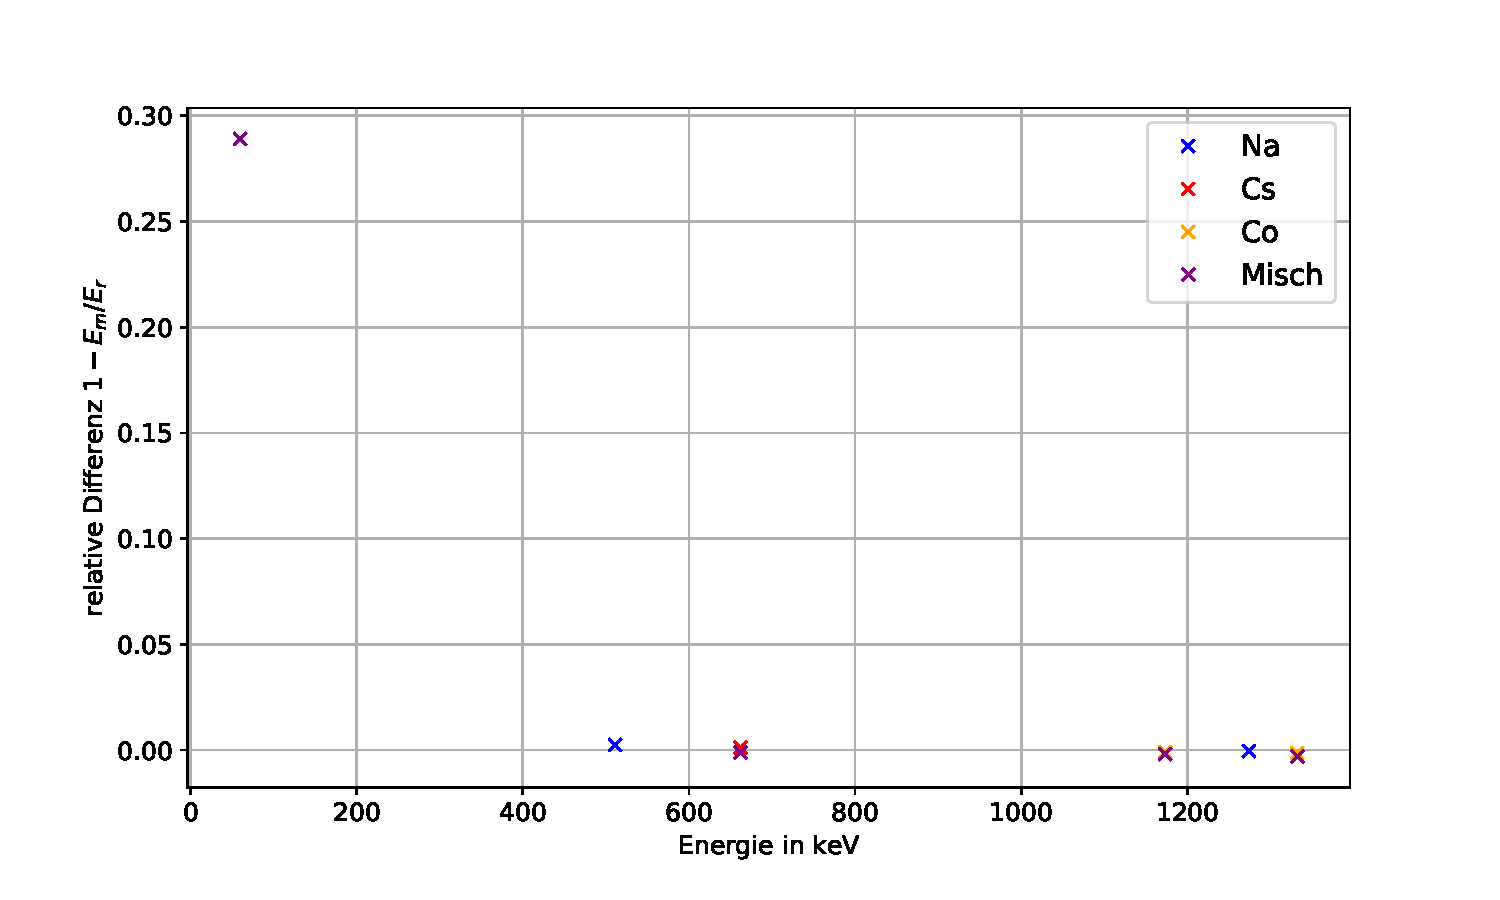
\includegraphics[width= \linewidth]{img/diff_na.pdf}
			\subcaption{
				relative Differenz.
			}
		\end{subfigure}
		\begin{subfigure}[t]{0.8\textwidth}
			\centering
			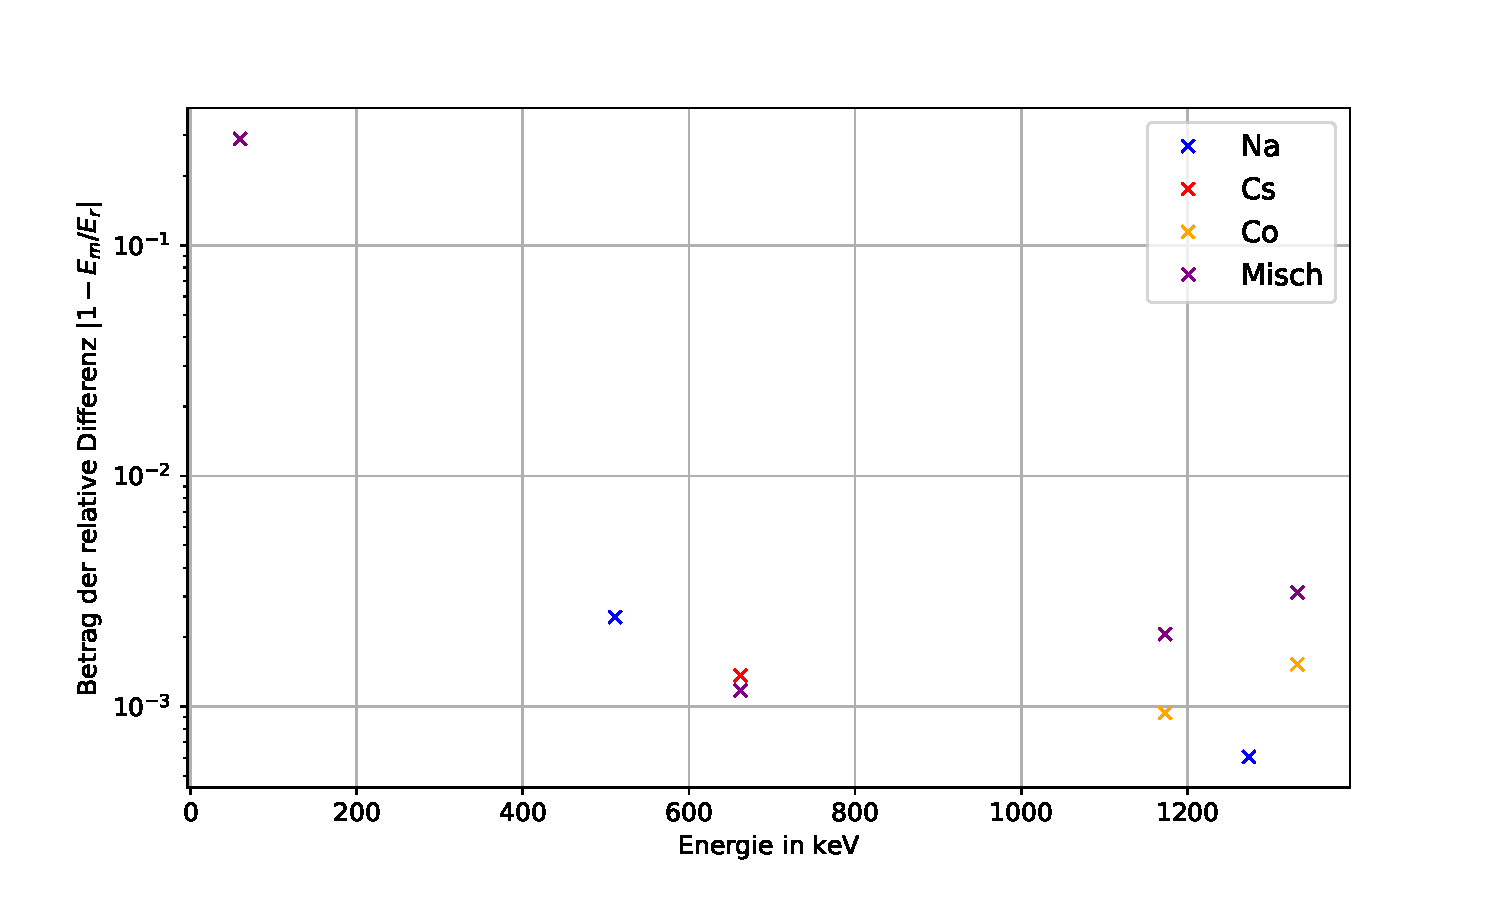
\includegraphics[width=\linewidth]{img/diff_na_log.pdf}
			\subcaption{
				Betrag der relativen Differenz in logarithmischer Darstellung.
			}
		\end{subfigure}
		\caption{Nichtlinearität des NaI-Detektors.
		Die Unsicherheiten sind nicht abgebildet, da ein Abbilden dieser ein Unterscheiden der Werte unmöglich macht. %TODO ...da sie im Vergleich sehr groß sind.
		Der Wert Null für die relative Differenz liegt immer im Unsicherheitsintervall.
		}
		\label{fg_diff_na}
	\end{figure}
\begin{figure}[H]
		\centering
		\begin{subfigure}[t]{0.8\textwidth}
			\centering
			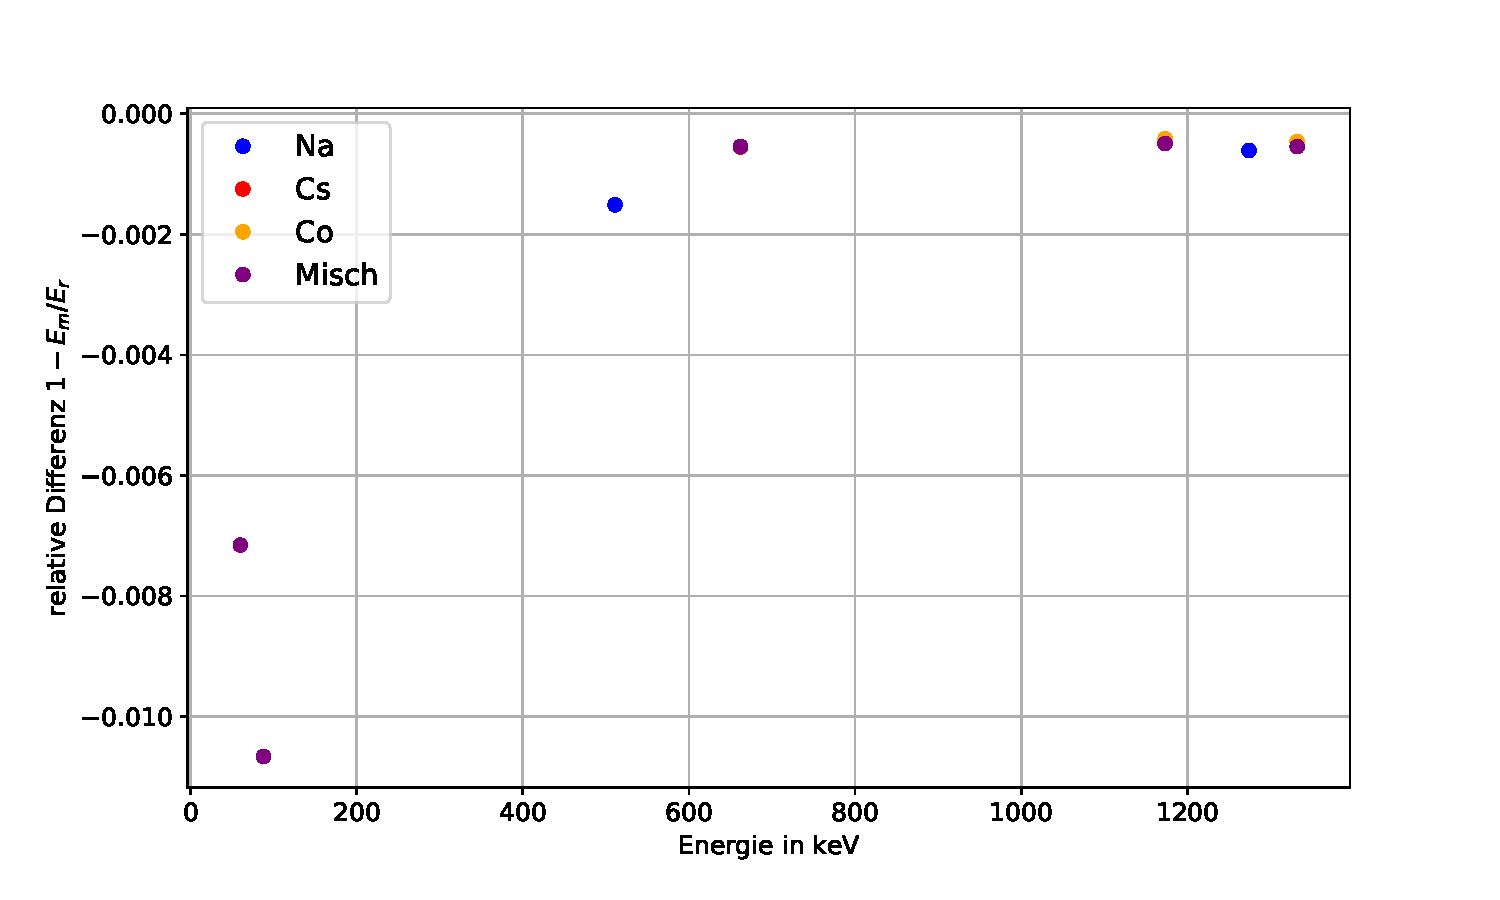
\includegraphics[width= \linewidth]{img/diff_ge.pdf}
			\subcaption{
				relative Differenz.
			}
		\end{subfigure}
		\begin{subfigure}[t]{0.8\textwidth}
			\centering
			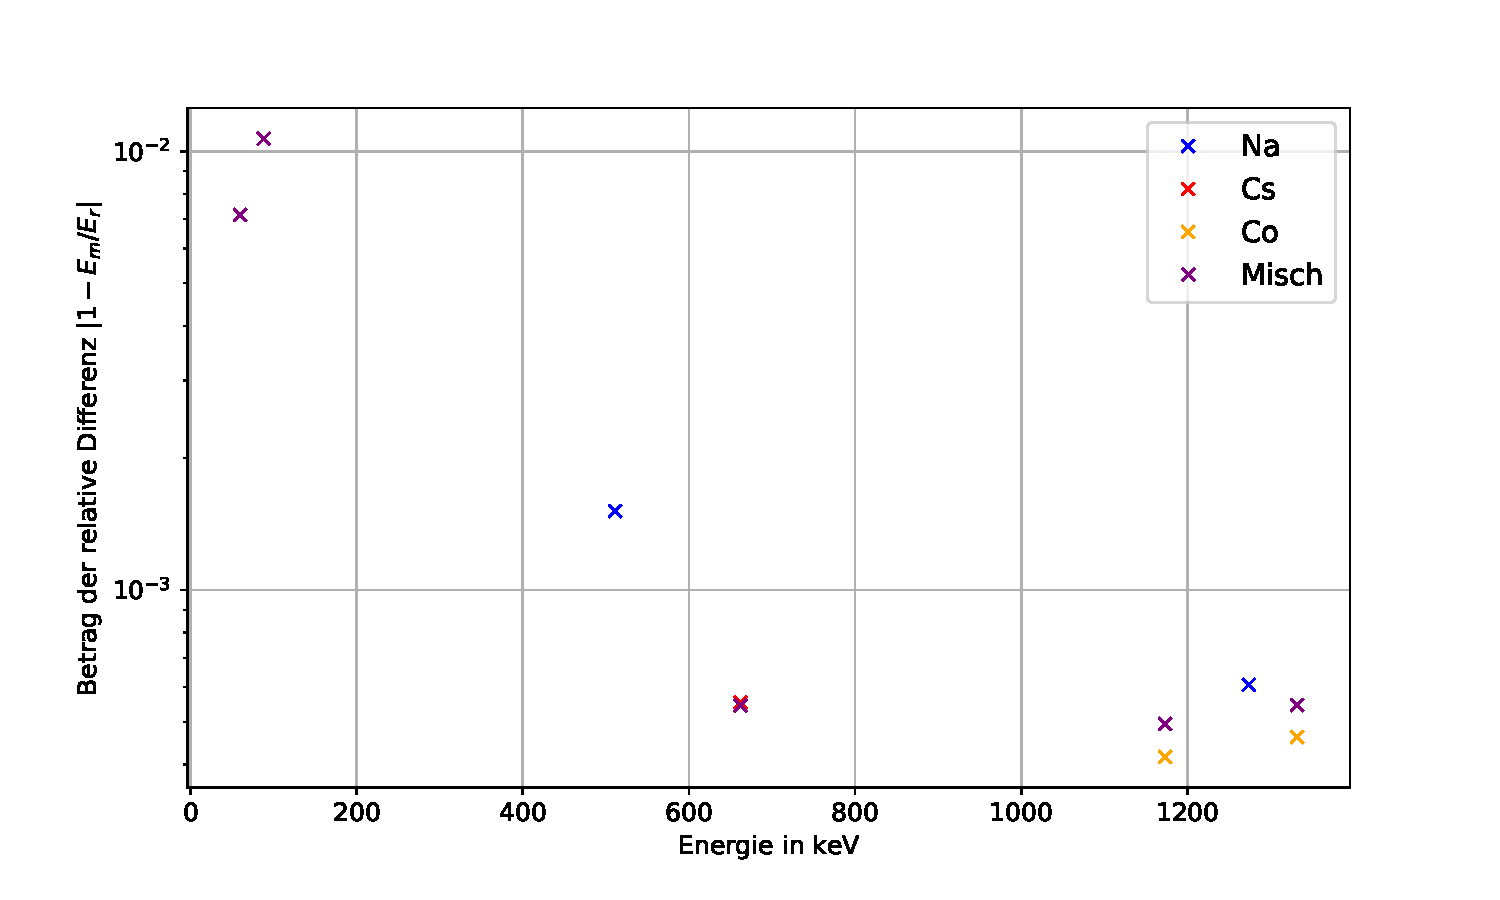
\includegraphics[width= \linewidth]{img/diff_ge_log.pdf}
			\subcaption{
				Betrag der relativen Differenz in logarithmischer Darstellung.
			}
		\end{subfigure}
		\caption{Nichtlinearität des Ge-Detektors.
		Die Unsicherheiten sind nicht abgebildet, da ein Abbilden dieser ein Unterscheiden der Werte unmöglich macht.
		Der Wert Null für die relative Differenz liegt immer im Unsicherheitsintervall.
		}
		\label{fg_diff_ge}
	\end{figure}
\subsection{Energieauflösung}
Die Energieauflösung $\Delta E$ lässt sich aus der Standardabweichung $\sigma$ und der Position $E$ eines Peaks berechnen.
Die Formel hierfür ist:
\begin{equation}
	\Delta E = \frac{\sigma}{E}
\end{equation}
Die Unsicherheiten für $\sigma$ ergeben sich aus der Multiplikation mit der Steigung $m$ aus der Kalibrationsgeradengleichung (\ref{eq_trans}).


	\begin{figure}[H]
			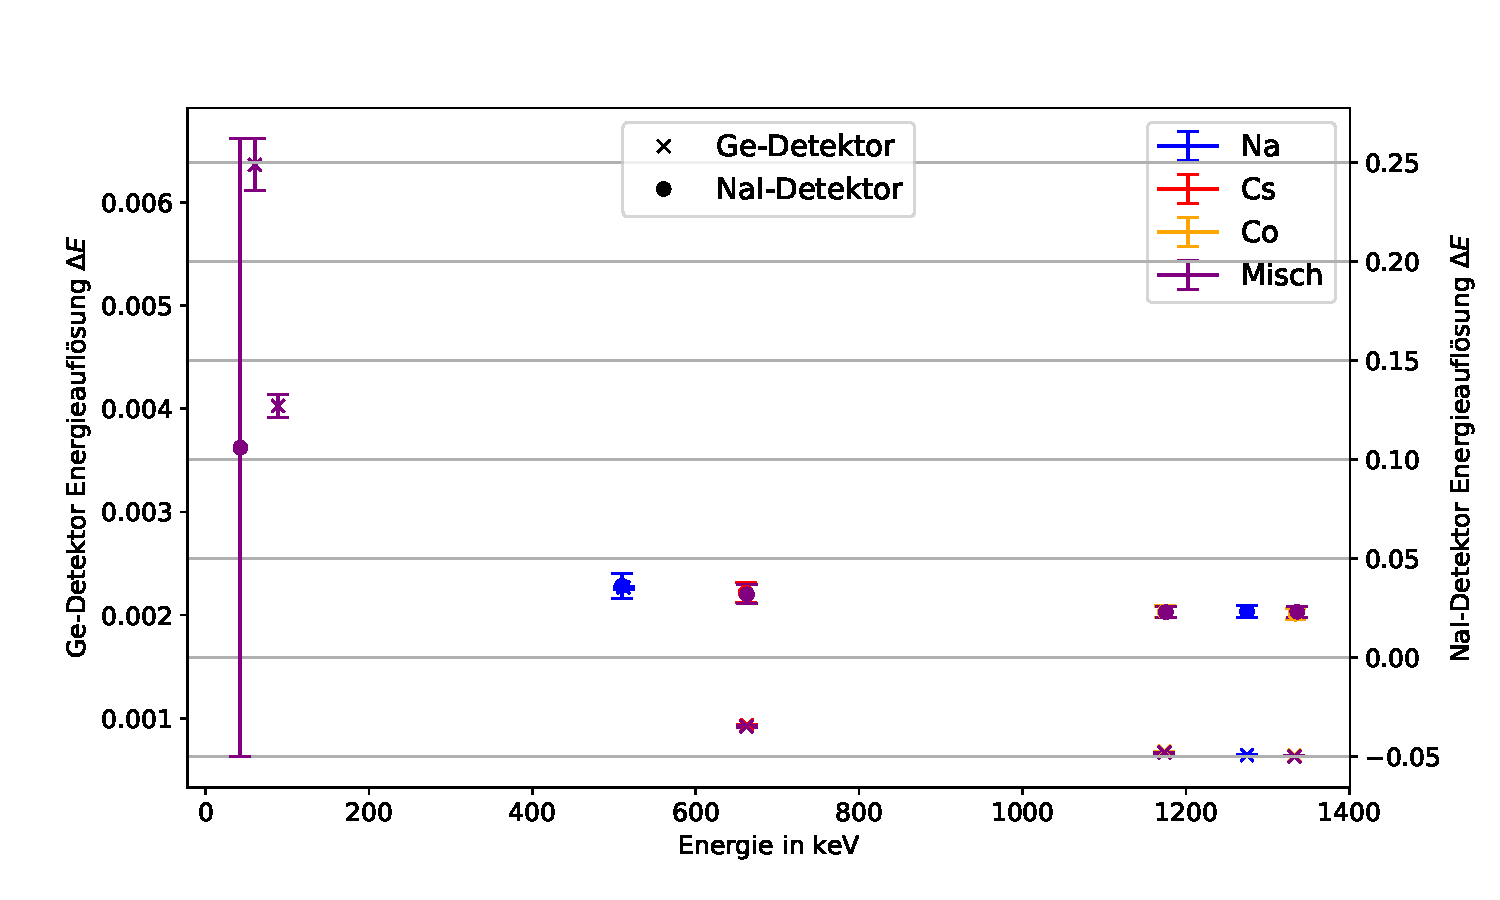
\includegraphics[width= 1 \linewidth]{img/res}
			\caption{
			Energieauflösung für NaI- und Ge-Detektor.
			}
			\label{fg_resolution}
	\end{figure}
%TODO Schon Diskussion?
Die große Unsicherheit des niederenergetischen NaI-Detektor Messpunkts ist der großen (relativen) Unsicherheit des ersten Peaks in der Mischprobe geschuldet (\cref{fg_Mix_Na}).
\subsection{Mittlere Ionisationsenergie}
Die Mittlere Ionisationsenergie $I$ lässt sich ebenso aus der Standardabweichung $\sigma$ und der Position $E$ eines Full-Energy-Peaks berechnen.
Die Formel hierfür ist:
%TODO Theo: explain calc
\begin{equation}
	I = \frac{\sigma^2}{E}
\end{equation}
Die Unsicherheiten für $\sigma$ ergeben sich aus der Multiplikation mit der Steigung $m$ aus der Kalibrationsgeradengleichung (\ref{eq_trans}).


	\begin{figure}[H]
			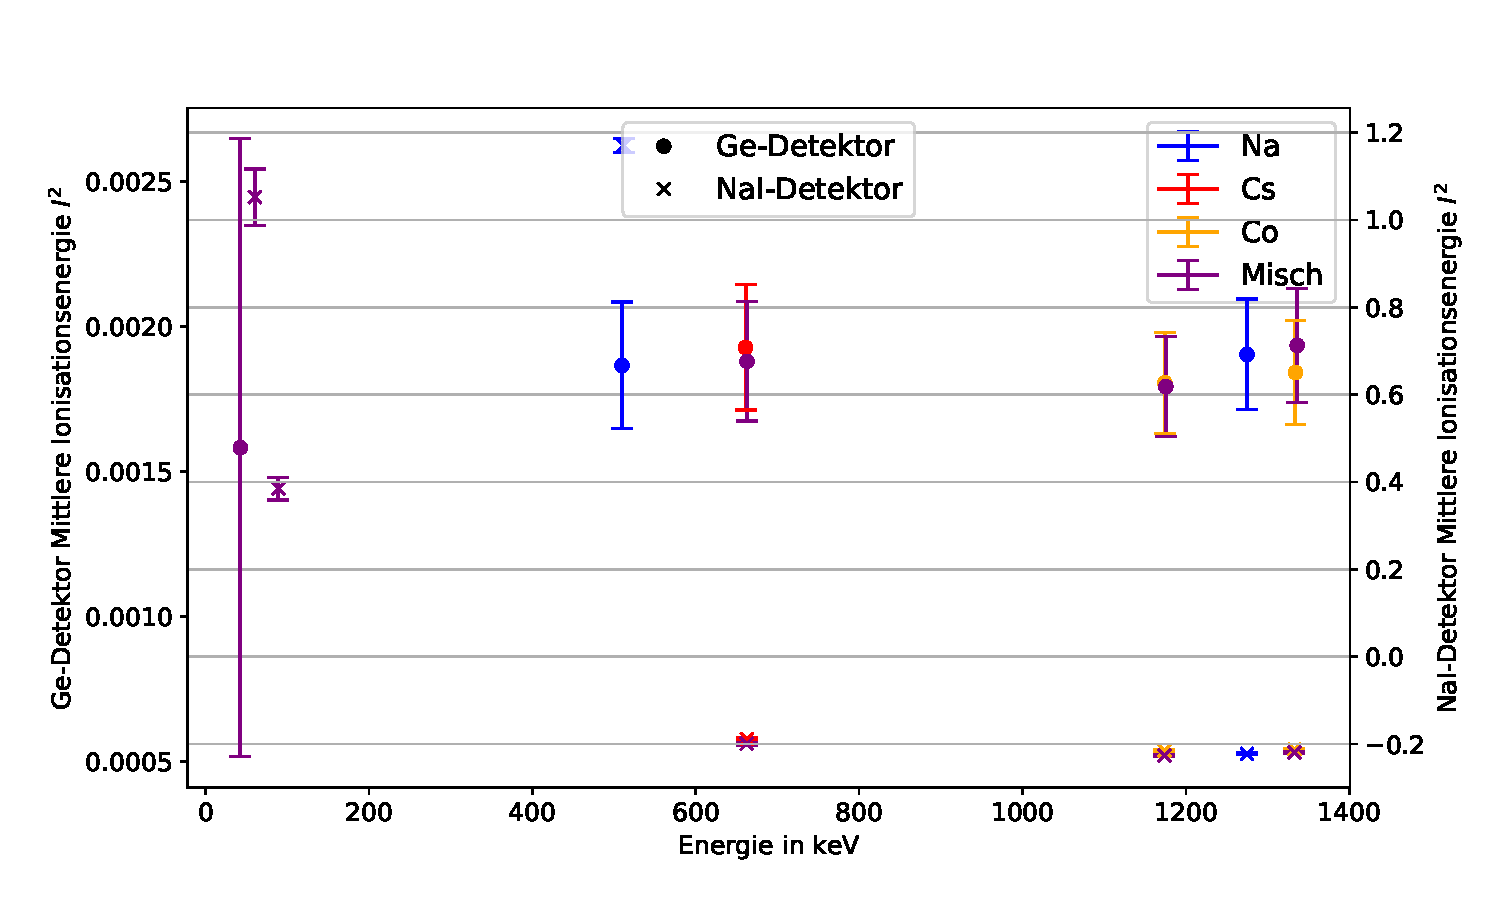
\includegraphics[width= 1 \linewidth]{img/ion}
			\caption{
			Mittlere Ionisationsenergie für NaI- und Ge-Detektor.
			}
			\label{fg_ionisation}
	\end{figure}
\subsection{Relative Effizienz}
Die relative normierte Effizienz $\varepsilon$ lässt sich nach \cref{eq_rel_eff} berechnen.
\begin{equation}
	\label{eq_rel_eff}
	\varepsilon = \frac{\frac{S}{P}}{\left|\frac{S}{P}\right|}_{\text{ref}}
\end{equation}
%TODO in Theorie: Full Energy Peak ETC.
Wobei $S$ die Fläche eines Full-Energy-Peak ist und $P$ die Anzahl Photonen, welche im Messzeitraum $t$ durch diesen $\gamma$-Übergang ausgesendet werden.
Dieses Verhältnis wird auf einen Messpunkt $\left|\frac{S}{P}\right|_{\text{ref}}$ normiert.
Die Anzahl Photonen ist das Produkt aus Messdauer $t$ und Aktivität $A$ des $\gamma$-Übergangs, $P=A\cdot t$.
Die derzeitige ($t'$) Aktivitäten wurden aus einer vorherigen ($t_r$) Messung und bekannter Zerfallskonstante $\lambda$ berechnet.
\begin{equation}
	A(t') = A(t_r)\exp^{-\lambda (t'-t_r)}
\end{equation}
Die Ergebnisse sind in \cref{fg_eff} gegen die Energie $E$ aufgetragen.
Als Normierung wurde für beide Detektoren der Full-Energy-Peak bei \SI{662}{keV} verwendet.

	\begin{figure}[H]
			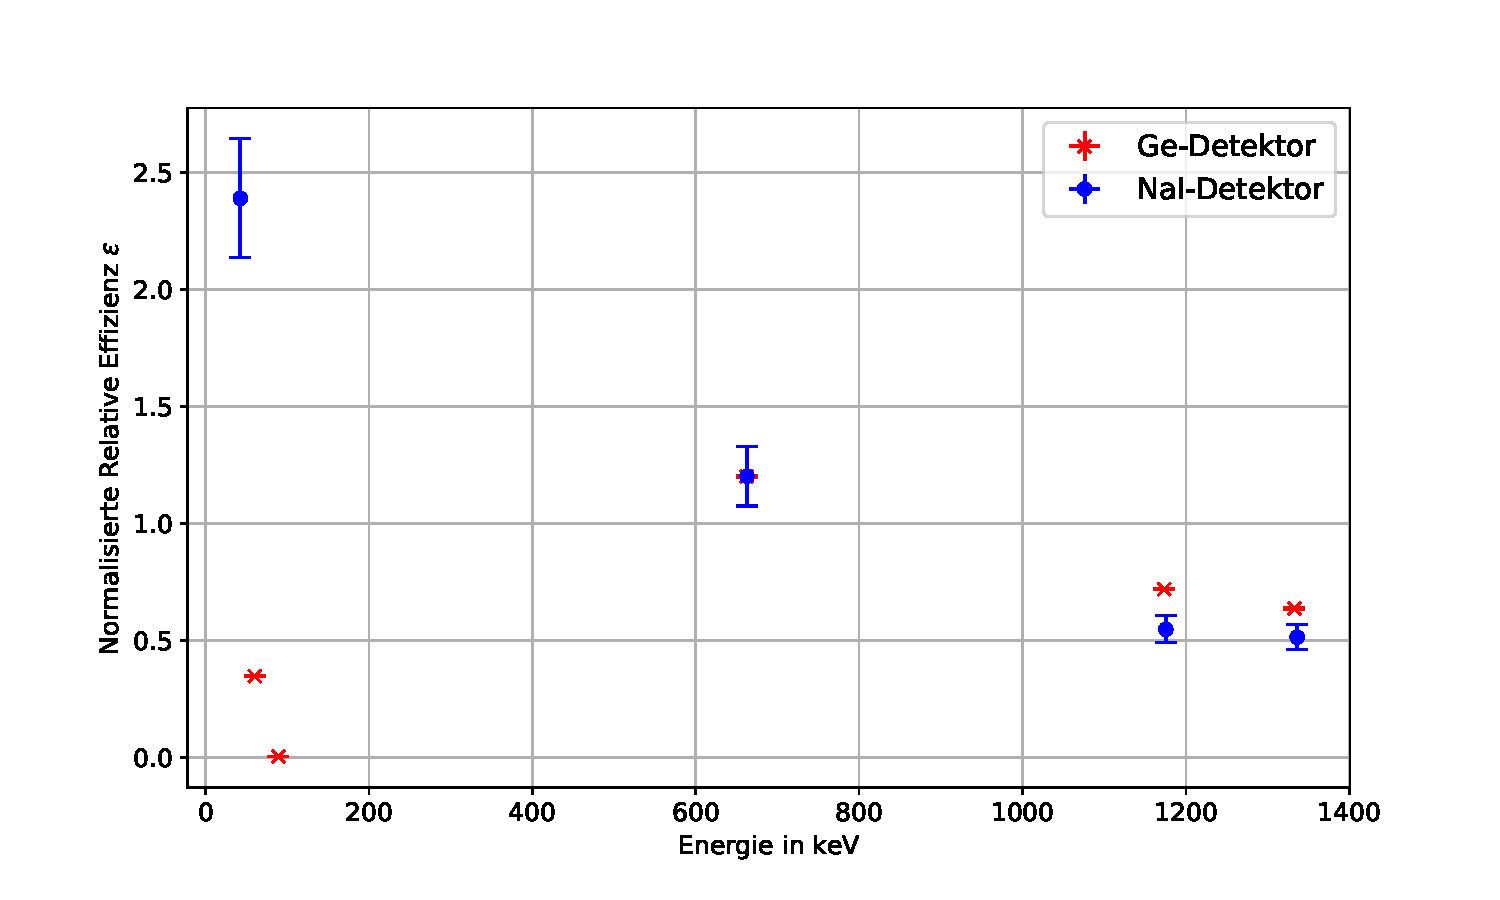
\includegraphics[width= 1 \linewidth]{img/eff}
			\caption{
			Normierte Relative Effizienz für NaI- und Ge-Detektor bei der Mischprobe.
			}
			\label{fg_eff}
	\end{figure}
	%TODO Diskuss: grund für hohe NaI-Wert: Auflösung zuschlecht für die zwei peaks die Ge da hat, stackt sich dann.
\subsection{Erzprobe}
	In \cref{fg_erz} ist das Spektrum der Erzprobe abgebildet.
	In unterschiedlichen Farben sind passende Peaks der vier natürlichen Zerfallsreihen markiert.
	Im \nameref{s_anhang} sind in \crefrange{fg_erz_np}{fg_erz_u_ra} die Zerfallsreihen separat markiert.
	Hierbei wurde nach Augemaß schwarz für ein passenden Peak, rot für ein verschobenen oder schwachen Peak, und blau für keine Korrelation verwendet.
	Die Literaturwerte für die Energien $E_\gamma$ stammen aus \cite{erze1} und \cite{erze2}.
	Es wurden direkt Peaks mit einer relativen Intensität kleiner \SI{5}{\percent} ausgeschlossen.

	\begin{figure}[H]
			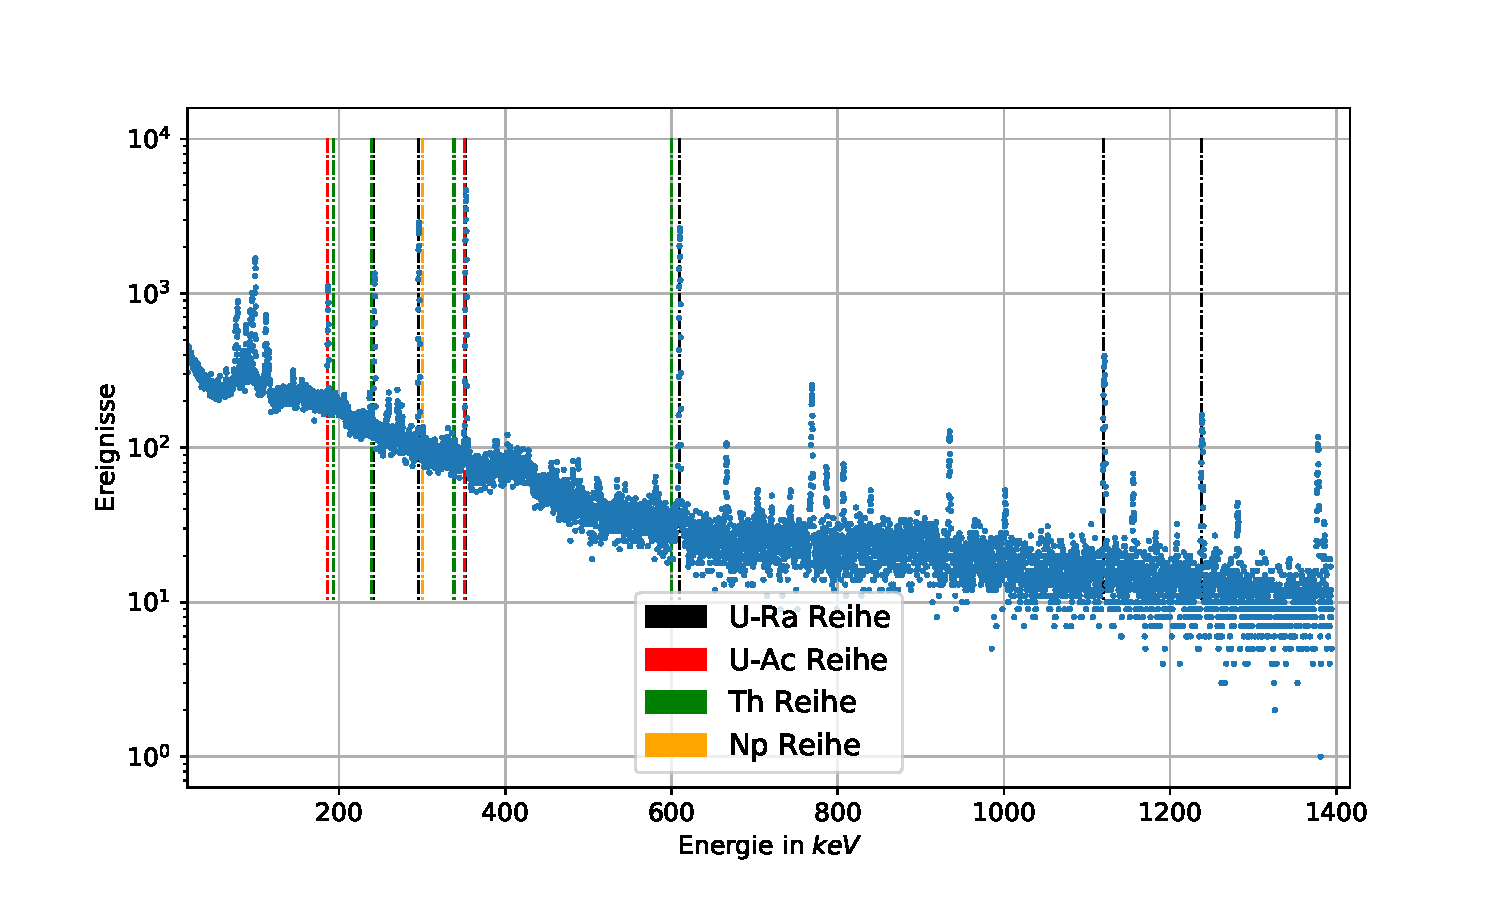
\includegraphics[width= 1 \linewidth]{img/erz_alles}
			\caption{
			Spektrum der Erzprobe. Einige passende $\gamma$-Übergangenergien sind von den vier Zerfallsreihen farblich eingezeichnet.
			}
			\label{fg_erz}
	\end{figure}
	%TODO U-Ra passt am besten

	\section{Diskussion}
	% Bezug/Nutzen oder sonst was
	% auch hier die Hypothese wiederholen
	% keine Messwerte hier, nach manchen Menschen, zumindest "direkt" erstellte Diagramme net hier, auch wenn Lesbarkeit-bla
	%TODO Rückstreuungsminimierung durch Deckel abnehmen aber immernoch Luft/Decke/we

	\subsection{Interpretation}
	%TODO features of typical gamma spectrum
	%TODO Vergleich Literaturwerte der gammalinien
	%TODO Vergleich Literaturwerte der comptonkanten
	%TODO zusätzliche Peaks zusehen?
	%TODO welche der erwarteten Peaks in der Mischprobe?
	%TODO welche Isotope in der unbekannten Probe? Zu welcher Zerfallsreihe gehören die.

	\subsection{Vergleich der Detektoren}
	%TODO Wie Energieunschärfe?
	%TODO Zusammenhang Energieauflösung und mittlere Ionisationsenergie?
	%TODO Abhängigkeit der beiden von Energie?
	%TODO Definition der Effizienz? Wie misst man das?
	%TODO Ist es möglich die Effizienzen zu vergleichen?->Raumgeometrie?
	%TODO Wo sind die Detektoren ähnlich?


	%TODO warum 511 nur bei NA?
	\section{Schlussfolgerung}
	% Rückgriff auf Hypothese und drittes Nennen dieser
	Insgesamt gesehen lässt sich sagen, dass
	%TODO Ergibnis Spektren-Aussehen
	%TODO Ergebnis Vergleich detektroen
	%TODO Ergebnis unbektannte Probe


	\section{Anhang} \label{s_anhang}

	\begin{figure}[H]
			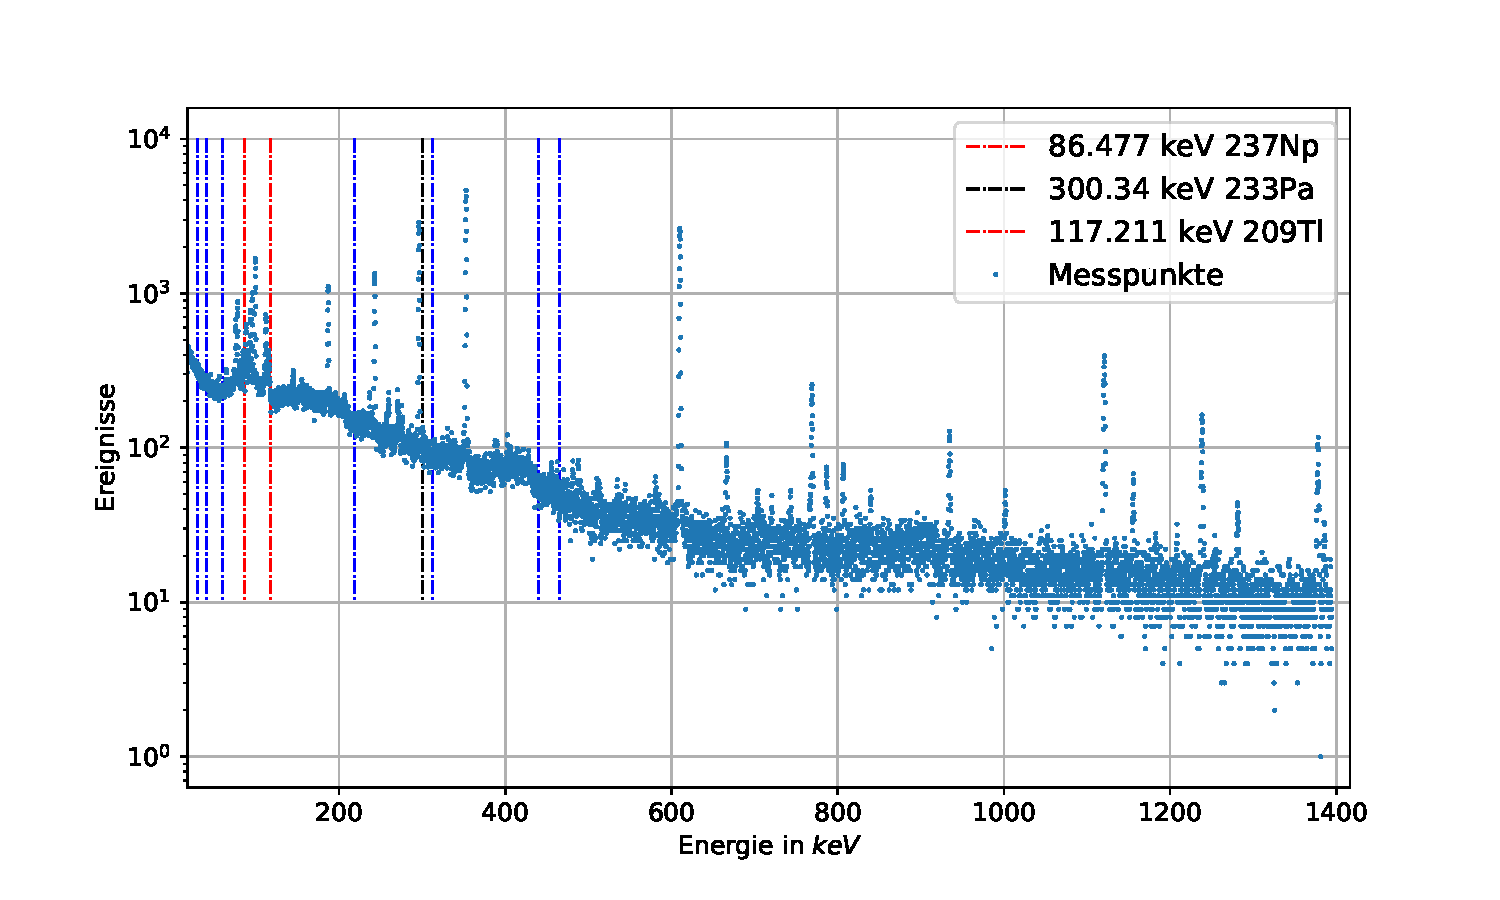
\includegraphics[width= 1 \linewidth]{img/erz_Np}
			\caption{
			Spektrum der Erzprobe. Np-Reihen $\gamma$-Übergangenergien sind von den vier Zerfallsreihen farblich eingezeichnet.
			}
			\label{fg_erz_np}
	\end{figure}
	\begin{figure}[H]
			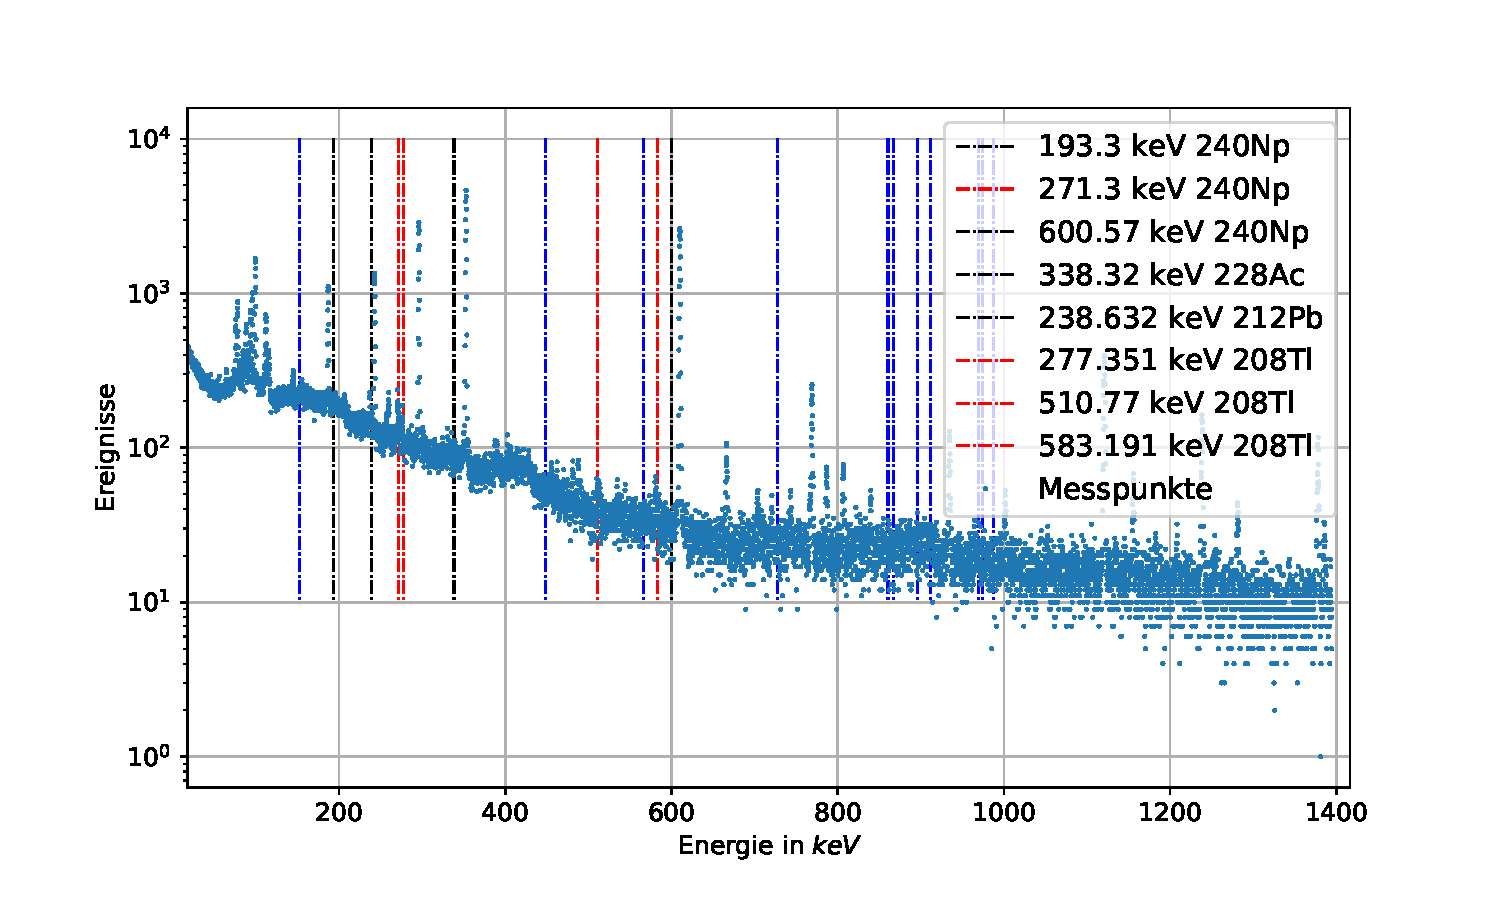
\includegraphics[width= 1 \linewidth]{img/erz_Th}
			\caption{
			Spektrum der Erzprobe. Th-Reihen $\gamma$-Übergangenergien sind von den vier Zerfallsreihen farblich eingezeichnet.
			}
			\label{fg_erz_th}
	\end{figure}
	\begin{figure}[H]
			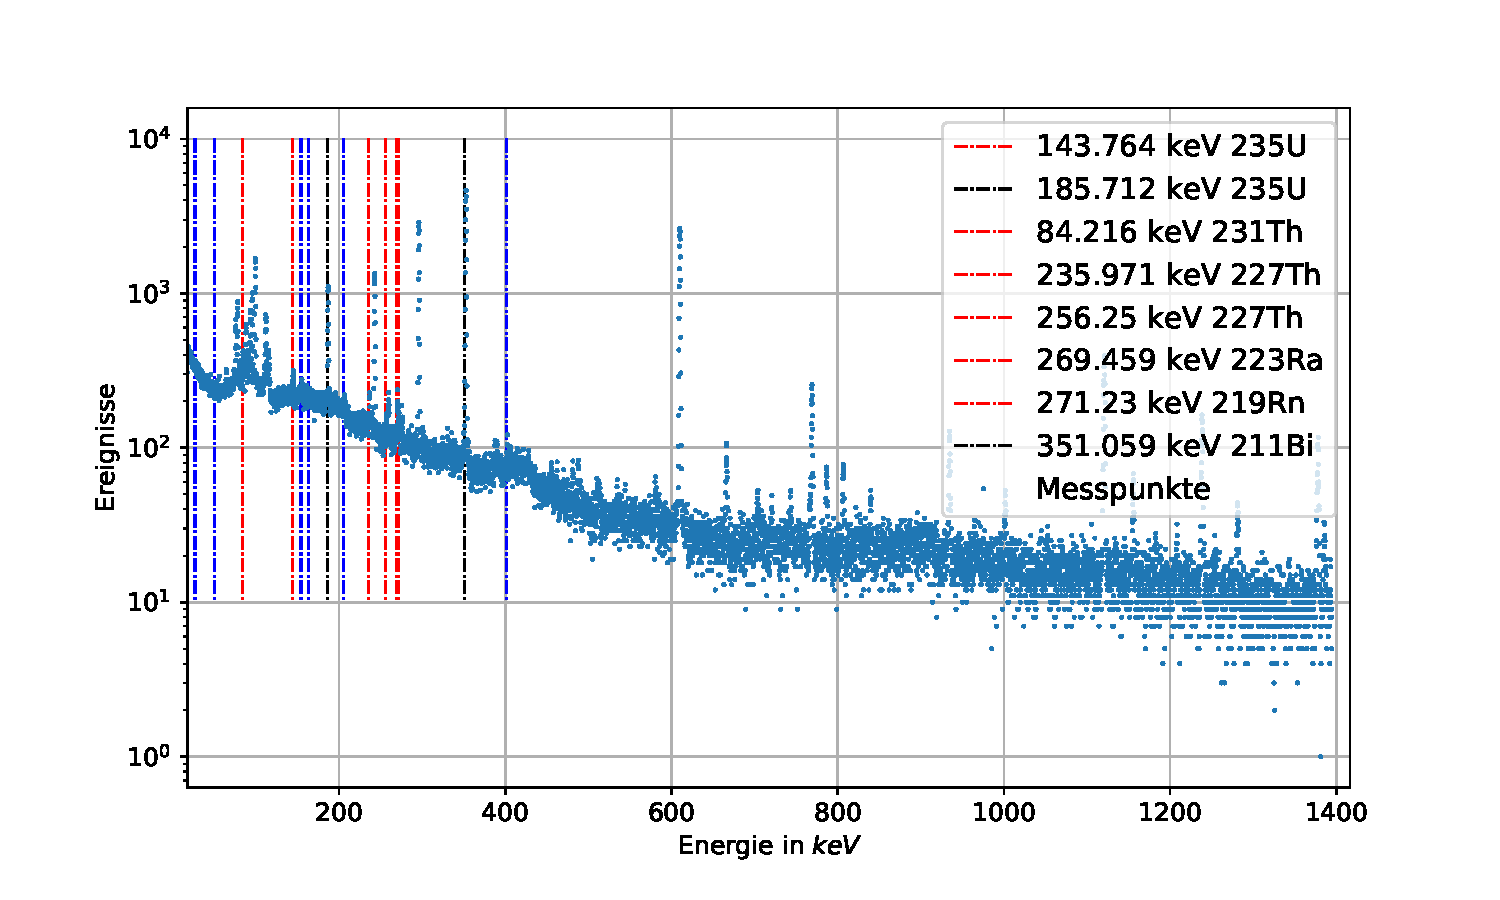
\includegraphics[width= 1 \linewidth]{img/erz_U-Ac}
			\caption{
			Spektrum der Erzprobe. $^{235}$U-Reihen $\gamma$-Übergangenergien sind von den vier Zerfallsreihen farblich eingezeichnet.
			}
			\label{fg_erz_u_ac}
	\end{figure}
	\begin{figure}[H]
			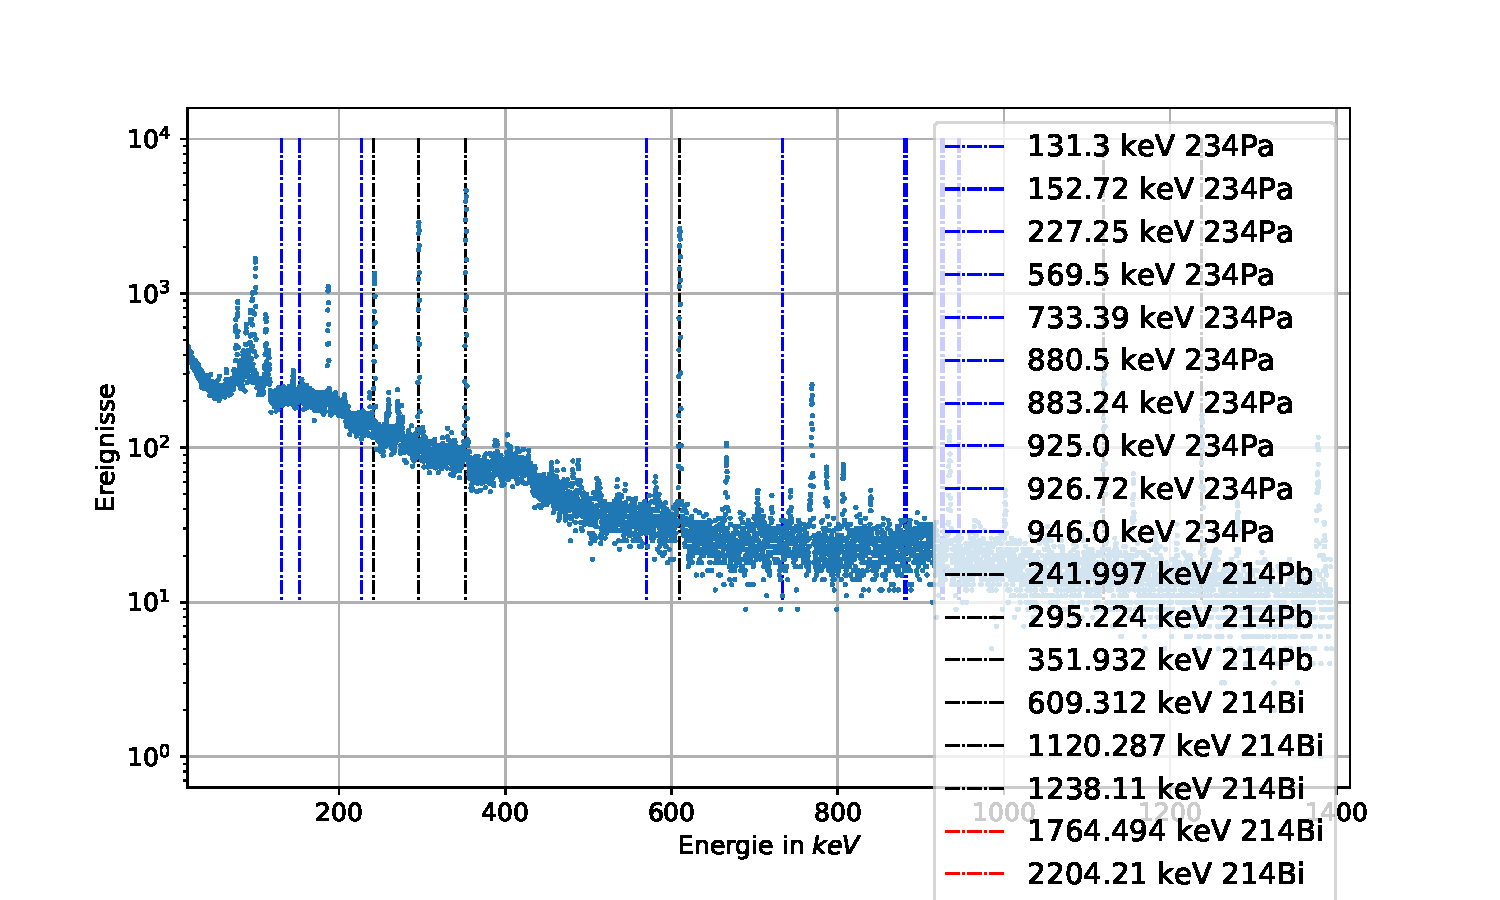
\includegraphics[width= 1 \linewidth]{img/erz_U-Ra}
			\caption{
			Spektrum der Erzprobe. $^{238}$U-Reihen $\gamma$-Übergangenergien sind von den vier Zerfallsreihen farblich eingezeichnet.
			}
			\label{fg_erz_u_ra}
	\end{figure}
	% Quellen zitieren, Websiten mit Zugriffsdatum
	% Verweise auf das Laborbuch (sind erlaubt)
	% Tabelle + Bilder mit Beschriftung
	\printbibliography
\end{document}

%TODO Ich hab der anleitung nen Datum gegeben, weil dass da drauf steht. Vielleicht ist nur das Jahr sinnvoller, weil mans bei veröffentlichungen so machen würde.
